\documentclass{article}




\usepackage{fullpage}
\usepackage{nopageno}
\usepackage{amsmath}
\usepackage{amsfonts}
\usepackage{graphicx}
\usepackage{framed}
\usepackage{algorithmic}
\usepackage{xcolor}

\definecolor{dark_red}{rgb}{0.5,0.0,0.0}
\definecolor{dark_green}{rgb}{0.0,0.5,0.0}
\definecolor{dark_blue}{rgb}{0.0,0.0,0.5}
\definecolor{blue}{rgb}{0.0,0.0,1.0}

\newcommand{\dr}[1]{\textcolor{dark_red}{#1}}
\newcommand{\dg}[1]{\textcolor{dark_green}{#1}}
\newcommand{\db}[1]{\textcolor{dark_blue}{#1}}
\newcommand{\blue}[1]{\textcolor{blue}{#1}}



\begin{document}



\section*{Subspaces of $\mathbb{R}^n$}

A set \(S\) of vectors from \(\mathbb{R}^n\) is a ``linear subspace" of \(\mathbb{R}^n\) if and only if the following properties hold.

Closure under addition and scalar multiplication:
\begin{itemize}
\item For all vectors \(\mathbf{u} \in S\) and \(\mathbf{v} \in S\), \(\mathbf{u} + \mathbf{v} \in S\). This is ``closure under addition".
\item For all vectors \(\mathbf{u} \in S\) and and scalars \(c \in \mathbb{R}\), \(c \mathbf{u} \in S\). This is ``closure under scalar multiplication", and is supported by, but not firmly proven from, closure under addition.
\item For all vectors \(\mathbf{u}_1, \mathbf{u}_2, ..., \mathbf{u}_k \in S\) and scalars \(c_1, c_2, ..., c_k \in \mathbb{R}\), 
\[c_1 \mathbf{u}_1 + c_2 \mathbf{u}_2 + ... + c_k \mathbf{u}_k \in S\] 
This directly follows from closure under addition and closure under scalar multiplication.
\end{itemize}

In the sections to follow, many examples of linear subspaces will be discussed. 

\textbf{Examples:}
\begin{itemize}
%%%%%%%%%%%%%%%%%%%%%%%%%%%%%
\item Consider the set \(S\) of \(3\)-component vectors where the last component is \(0\):
\[S = \left\{\begin{bmatrix} x \\ y \\ 0 \end{bmatrix}\middle| x, y \in \mathbb{R} \right\}\]
Is \(S\) a linear subspace? 

Firstly, closure under addition should be tested:
Let \(\mathbf{u}\) and \(\mathbf{v}\) denote two arbitrary vectors from \(S\). Let \(\mathbf{u} = \begin{bmatrix} u_x \\ u_y \\ 0 \end{bmatrix}\) and \(\mathbf{v} = \begin{bmatrix} v_x \\ v_y \\ 0 \end{bmatrix}\).
\[\mathbf{u} + \mathbf{v} = \begin{bmatrix} u_x \\ u_y \\ 0 \end{bmatrix} + \begin{bmatrix} v_x \\ v_y \\ 0 \end{bmatrix} = \begin{bmatrix} u_x + v_x \\ u_y + v_y \\ 0 \end{bmatrix}\]
The last component is \(0\), so \(\mathbf{u} + \mathbf{v} \in S\) and there is closure under addition. 

Next, closure under scalar multiplication is to be tested:
Let \(\mathbf{u}\) denote an arbitrary vector from \(S\), and let \(c\) denote an arbitrary scalar. Let \(\mathbf{u} = \begin{bmatrix} u_x \\ u_y \\ 0 \end{bmatrix}\). 
\[c\mathbf{u} = c\begin{bmatrix} u_x \\ u_y \\ 0 \end{bmatrix} = \begin{bmatrix} c u_x \\ c u_y \\ 0 \end{bmatrix}\] 
The last component is \(0\), so \(c \mathbf{u} \in S\) and there is closure under scalar multiplication. 

There is closure under both addition and scalar multiplication so \(S\) is therefore a linear subspace. 
%%%%%%%%%%%%%%%%%%%%%%%%%%%%%
\item Consider the set \(S\) of \(3\)-component vectors where the last component is \(-2\):
\[S = \left\{\begin{bmatrix} x \\ y \\ -2 \end{bmatrix}\middle| x, y \in \mathbb{R} \right\}\]
Is \(S\) a linear subspace? 

Firstly, closure under addition should be tested:
Let \(\mathbf{u}\) and \(\mathbf{v}\) denote two arbitrary vectors from \(S\). Let \(\mathbf{u} = \begin{bmatrix} u_x \\ u_y \\ -2 \end{bmatrix}\) and \(\mathbf{v} = \begin{bmatrix} v_x \\ v_y \\ -2 \end{bmatrix}\).
\[\mathbf{u} + \mathbf{v} = \begin{bmatrix} u_x \\ u_y \\ -2 \end{bmatrix} + \begin{bmatrix} v_x \\ v_y \\ -2 \end{bmatrix} = \begin{bmatrix} u_x + v_x \\ u_y + v_y \\ -4 \end{bmatrix}\]
The last component is \(-4\), so \(\mathbf{u} + \mathbf{v} \notin S\) and there is no closure under addition. 

There is no closure under addition and \(S\) is therefore not a linear subspace.
%%%%%%%%%%%%%%%%%%%%%%%%%%%%%
\item Consider the following set \(S\) of \(2\)-component vectors:
\[S = \left\{\begin{bmatrix} x \\ y \end{bmatrix}\middle| x, y \in \mathbb{R} \;\;\text{and}\;\; y = -5x \right\}\]
Is \(S\) a linear subspace? 

Firstly, closure under addition should be tested:
Let \(\mathbf{u}\) and \(\mathbf{v}\) denote two arbitrary vectors from \(S\). Let \(\mathbf{u} = \begin{bmatrix} u_x \\ u_y \end{bmatrix}\) and \(\mathbf{v} = \begin{bmatrix} v_x \\ v_y \end{bmatrix}\) where \(u_y = -5u_x\) and \(v_y = -5v_x\).
\[\mathbf{u} + \mathbf{v} = \begin{bmatrix} u_x \\ u_y \end{bmatrix} + \begin{bmatrix} v_x \\ v_y \end{bmatrix} = \begin{bmatrix} u_x + v_x \\ u_y + v_y \end{bmatrix}\]
\[u_y + v_y = (-5u_x) + (-5v_x) = -5(u_x + v_x)\]
so \(\mathbf{u} + \mathbf{v} \in S\) and there is closure under addition. 

Next, closure under scalar multiplication is to be tested:
Let \(\mathbf{u}\) denote an arbitrary vector from \(S\), and let \(c\) denote an arbitrary scalar. Let \(\mathbf{u} = \begin{bmatrix} u_x \\ u_y \end{bmatrix}\) where \(u_y = -5u_x\). 
\[c\mathbf{u} = c\begin{bmatrix} u_x \\ u_y \end{bmatrix} = \begin{bmatrix} c u_x \\ c u_y \end{bmatrix}\] 
\[c u_y = c(-5u_x) = -5(c u_x)\]
so \(c \mathbf{u} \in S\) and there is closure under scalar multiplication. 

There is closure under both addition and scalar multiplication so \(S\) is therefore a linear subspace. 
%%%%%%%%%%%%%%%%%%%%%%%%%%%%%
\item Consider the following set \(S\) of \(2\)-component vectors:
\[S = \left\{\begin{bmatrix} x \\ y \end{bmatrix}\middle| x, y \in \mathbb{R} \;\;\text{and}\;\; x+y=5 \right\}\]
Is \(S\) a linear subspace? 

Firstly, closure under addition should be tested:
Let \(\mathbf{u}\) and \(\mathbf{v}\) denote two arbitrary vectors from \(S\). Let \(\mathbf{u} = \begin{bmatrix} u_x \\ u_y \end{bmatrix}\) and \(\mathbf{v} = \begin{bmatrix} v_x \\ v_y \end{bmatrix}\) where \(u_x + u_y = 5\) and \(v_x + v_y = 5\).
\[\mathbf{u} + \mathbf{v} = \begin{bmatrix} u_x \\ u_y \end{bmatrix} + \begin{bmatrix} v_x \\ v_y \end{bmatrix} = \begin{bmatrix} u_x + v_x \\ u_y + v_y \end{bmatrix}\]
\[(u_x + v_x) + (u_y + v_y) = (u_x + u_y) + (v_x + v_y) = 5 + 5 = 10\]
so \(\mathbf{u} + \mathbf{v} \notin S\) and there is no closure under addition. 

There is no closure under addition and \(S\) is therefore not a linear subspace.
%%%%%%%%%%%%%%%%%%%%%%%%%%%%%
\item Consider the following set \(S\) of \(2\)-component vectors:
\[S = \left\{\begin{bmatrix} x \\ y \end{bmatrix}\middle| x, y \in \mathbb{R} \;\;\text{and}\;\; x \geq 0 \right\}\]
Is \(S\) a linear subspace? 

Firstly, closure under addition should be tested:
Let \(\mathbf{u}\) and \(\mathbf{v}\) denote two arbitrary vectors from \(S\). Let \(\mathbf{u} = \begin{bmatrix} u_x \\ u_y \end{bmatrix}\) and \(\mathbf{v} = \begin{bmatrix} v_x \\ v_y \end{bmatrix}\) where \(u_x \geq 0\) and \(v_x \geq 0\).
\[\mathbf{u} + \mathbf{v} = \begin{bmatrix} u_x \\ u_y \end{bmatrix} + \begin{bmatrix} v_x \\ v_y \end{bmatrix} = \begin{bmatrix} u_x + v_x \\ u_y + v_y \end{bmatrix}\]
From \(u_x \geq 0\) and \(v_x \geq 0\), \(u_x + v_x \geq 0\) so \(\mathbf{u} + \mathbf{v} \in S\) and there is closure under addition. 

Next, closure under scalar multiplication is to be tested:
Let \(\mathbf{u}\) denote an arbitrary vector from \(S\), and let \(c\) denote an arbitrary scalar. Let \(\mathbf{u} = \begin{bmatrix} u_x \\ u_y \end{bmatrix}\) where \(u_x \geq 0\). 
\[c\mathbf{u} = c\begin{bmatrix} u_x \\ u_y \end{bmatrix} = \begin{bmatrix} c u_x \\ c u_y \end{bmatrix}\] 
From \(u_x \geq 0\) it is not necessarily the case that \(c u_x \geq 0\), especially if \(c < 0\). It may not be the case that \(c u_x \geq 0\) so there is no closure under scalar multiplication. 

While there is closure under addition, there is no closure under scalar multiplication and \(S\) is therefore not a linear subspace.
%%%%%%%%%%%%%%%%%%%%%%%%%%%%%
\end{itemize}

One of the most common ways of quantifying a linear subspace is using a ``spanning set". 



\section*{Spanning sets}

Given an arbitrary set of vectors \(A = \{\mathbf{u}_1, \mathbf{u}_2, ..., \mathbf{u}_k\}\), the set of all vectors that are linear combinations of the vectors from \(A\) form a subspace referred to as the {\bf span} of \(A\), and is denoted by \(\text{span}(A)\). The linear subspace \(S = \text{span}(A)\) is also said to be {\bf generated} from \(A\). The set \(A\) is referred to as a {\bf spanning set} for \(S = \text{span}(A)\). The set \(A\) is said to {\bf span} the linear subspace \(S = \text{span}(A)\).  

A vector \(\mathbf{v}\) belongs to set \(\text{span}(A)\) if and only if there exists coefficients \(c_1, c_2, ..., c_k\) such that \(\mathbf{v} = c_1\mathbf{u}_1 + c_2\mathbf{u}_2 + ... + c_k\mathbf{u}_k\).  

%Let \(S\) be a ``subspace" of \(\mathbb{R}^n\). Given a set of vectors from \(S\): \(A = \{\mathbf{u}_1, \mathbf{u}_2, ..., \mathbf{u}_k\}\), this set of vectors is referred to as a ``spanning set" of \(S\) if and only if all vectors from \(S\), and only the vectors from \(S\), can be expressed as a linear combination of the vectors from the set \(A\):

It is fairly straightforwards to prove that \(\text{span}(A)\) is a linear subspace of \(\mathbb{R}^n\). 

Firstly, closure under addition must be proven. Let \(\mathbf{v}\) and \(\mathbf{w}\) denote two (not necessarily distinct) vectors from \(\text{span}(A)\). There must exist coefficients \(c_1, c_2, ..., c_k\) and \(d_1, d_2, ..., d_k\) such that: 
\[\mathbf{v} = c_1\mathbf{u}_1 + c_2\mathbf{u}_2 + ... + c_k\mathbf{u}_k \quad\text{and}\quad \mathbf{w} = d_1\mathbf{u}_1 + d_2\mathbf{u}_2 + ... + d_k\mathbf{u}_k\]

\[\mathbf{v} + \mathbf{w} = (c_1 + d_1)\mathbf{u}_1 + (c_2 + d_2)\mathbf{u}_2 + ... + (c_k + d_k)\mathbf{u}_k\]

Since \(\mathbf{v} + \mathbf{w}\) is a linear combination of the vectors from \(A\), \(\mathbf{v} + \mathbf{w} \in \text{span}(A)\), which makes \(\text{span}(A)\) closed under addition. 

Next, closure under scalar multiplication must be proven. Let \(\mathbf{v}\) denote an arbitrary vector from \(\text{span}(A)\), and let \(d\) denote an arbitrary scalar. There must exist coefficients \(c_1, c_2, ..., c_k\) such that: 
\[\mathbf{v} = c_1\mathbf{u}_1 + c_2\mathbf{u}_2 + ... + c_k\mathbf{u}_k\]

\[d \cdot \mathbf{v} = (d \cdot c_1)\mathbf{u}_1 + (d \cdot c_2)\mathbf{u}_2 + ... + (d \cdot c_k)\mathbf{u}_k\]

Since \(d \cdot \mathbf{v}\) is a linear combination of the vectors from \(A\), \(d \cdot \mathbf{v} \in \text{span}(A)\), which makes \(\text{span}(A)\) closed under scalar multiplication.

Therefore \(\text{span}(A)\) is a linear subspace. {\bf Moreover, every linear subspace is the span of some set of vectors.}

Of interest is the span of the empty set of vectors. When there are no vectors to use to build linear combinations, the span consists of only the zero vector:
\[\text{span}\{\} = \{\mathbf{0}\}\]
The ``empty" linear combination defaults to \(\mathbf{0}\). This technicality will become important when it is time to discuss basis sets, null spaces, and column spaces.



\textbf{Examples:}
\begin{itemize}
%%%%%%%%%%%%%%%%%%%%%%%%%
\item Does: \(\begin{bmatrix} 4 \\ 0 \\ 4 \end{bmatrix} \in \text{span}\left\{\begin{bmatrix} 1 \\ -1 \\ 2 \end{bmatrix}, \begin{bmatrix} 3 \\ -1 \\ 4 \end{bmatrix}\right\}\)?  

For \(\begin{bmatrix} 4 \\ 0 \\ 4 \end{bmatrix} \in \text{span}\left\{\begin{bmatrix} 1 \\ -1 \\ 2 \end{bmatrix}, \begin{bmatrix} 3 \\ -1 \\ 4 \end{bmatrix}\right\}\), the vector \(\mathbf{v} = \begin{bmatrix} 4 \\ 0 \\ 4 \end{bmatrix}\) must be a linear combination of the vectors \(\mathbf{u}_1 = \begin{bmatrix} 1 \\ -1 \\ 2 \end{bmatrix}\) and \(\mathbf{u}_2 = \begin{bmatrix} 3 \\ -1 \\ 4 \end{bmatrix}\): \(\mathbf{v} = c_1\mathbf{u}_1 + c_2\mathbf{u}_2\) for some coefficients \(c_1\) and \(c_2\).

\begin{align*}
& c_1\begin{bmatrix} 1 \\ -1 \\ 2 \end{bmatrix} + c_2\begin{bmatrix} 3 \\ -1 \\ 4 \end{bmatrix} = \begin{bmatrix} 4 \\ 0 \\ 4 \end{bmatrix}   
\iff \begin{bmatrix}
1 & 3 \\ 
-1 & -1 \\ 
2 & 4 
\end{bmatrix}\begin{bmatrix}
c_1 \\ c_2 
\end{bmatrix} = \begin{bmatrix} 4 \\ 0 \\ 4 \end{bmatrix}
\end{align*}   
Solving this system gives the following row reduction:
\begin{align*}
\left[\begin{array}{cc|c}
1 & 3 & 4 \\ 
-1 & -1 & 0 \\
2 & 4 & 4
\end{array}\right] 
\xrightarrow{\begin{array}{c} R_2 \rightarrow R_2 + R_1 \\ R_3 \rightarrow R_3 - 2R_1 \end{array}}  
\left[\begin{array}{cc|c}
1 & 3 & 4 \\ 
0 & 2 & 4 \\
0 & -2 & -4
\end{array}\right] 
\xrightarrow{\begin{array}{c} R_3 \rightarrow R_3 + R_2 \end{array}}  
\left[\begin{array}{cc|c}
1 & 3 & 4 \\ 
0 & 2 & 4 \\
0 & 0 & 0
\end{array}\right] 
\end{align*}
There is no pivot in the augmented column, so a solution exists, and hence:
\[\begin{bmatrix} 4 \\ 0 \\ 4 \end{bmatrix} \in \text{span}\left\{\begin{bmatrix} 1 \\ -1 \\ 2 \end{bmatrix}, \begin{bmatrix} 3 \\ -1 \\ 4 \end{bmatrix}\right\}\]  
%%%%%%%%%%%%%%%%%%%%%%%%%
\item Does: \(\begin{bmatrix} 5 \\ 5 \\ 5 \end{bmatrix} \in \text{span}\left\{\begin{bmatrix} 1 \\ -1 \\ 2 \end{bmatrix}, \begin{bmatrix} 3 \\ -1 \\ 4 \end{bmatrix}\right\}\)?  
\end{itemize}

For \(\begin{bmatrix} 5 \\ 5 \\ 5 \end{bmatrix} \in \text{span}\left\{\begin{bmatrix} 1 \\ -1 \\ 2 \end{bmatrix}, \begin{bmatrix} 3 \\ -1 \\ 4 \end{bmatrix}\right\}\), the vector \(\mathbf{v} = \begin{bmatrix} 5 \\ 5 \\ 5 \end{bmatrix}\) must be a linear combination of the vectors \(\mathbf{u}_1 = \begin{bmatrix} 1 \\ -1 \\ 2 \end{bmatrix}\) and \(\mathbf{u}_2 = \begin{bmatrix} 3 \\ -1 \\ 4 \end{bmatrix}\): \(\mathbf{v} = c_1\mathbf{u}_1 + c_2\mathbf{u}_2\) for some coefficients \(c_1\) and \(c_2\).

\begin{align*}
& c_1\begin{bmatrix} 1 \\ -1 \\ 2 \end{bmatrix} + c_2\begin{bmatrix} 3 \\ -1 \\ 4 \end{bmatrix} = \begin{bmatrix} 5 \\ 5 \\ 5 \end{bmatrix}   
\iff \begin{bmatrix}
1 & 3 \\ 
-1 & -1 \\ 
2 & 4 
\end{bmatrix}\begin{bmatrix}
c_1 \\ c_2 
\end{bmatrix} = \begin{bmatrix} 5 \\ 5 \\ 5 \end{bmatrix}
\end{align*}   
Solving this system gives the following row reduction:
\begin{align*}
\left[\begin{array}{cc|c}
1 & 3 & 5 \\ 
-1 & -1 & 5 \\
2 & 4 & 5
\end{array}\right] 
\xrightarrow{\begin{array}{c} R_2 \rightarrow R_2 + R_1 \\ R_3 \rightarrow R_3 - 2R_1 \end{array}}  
\left[\begin{array}{cc|c}
1 & 3 & 5 \\ 
0 & 2 & 10 \\
0 & -2 & -5
\end{array}\right] 
\xrightarrow{\begin{array}{c} R_3 \rightarrow R_3 + R_2 \end{array}}  
\left[\begin{array}{cc|c}
1 & 3 & 4 \\ 
0 & 2 & 4 \\
0 & 0 & 5
\end{array}\right] 
\end{align*}
There is a pivot in the augmented column, so no solution exists, and hence:
\[\begin{bmatrix} 5 \\ 5 \\ 5 \end{bmatrix} \notin \text{span}\left\{\begin{bmatrix} 1 \\ -1 \\ 2 \end{bmatrix}, \begin{bmatrix} 3 \\ -1 \\ 4 \end{bmatrix}\right\}\]  




\section*{Linear Independence}

When considering the span of a set of vectors \(A = \{\mathbf{u}_1, \mathbf{u}_2, ..., \mathbf{u}_k\}\), \(\text{span}\{\mathbf{u}_1, \mathbf{u}_2, ..., \mathbf{u}_k\}\), some of the vectors in the spanning set \(A\) may not be necessary. 

For example, let \(\mathbf{u}_1 = \begin{bmatrix} -3 \\ 2 \end{bmatrix}\), \(\mathbf{u}_2 = \begin{bmatrix} 7 \\ 1 \end{bmatrix}\), and \(\mathbf{u}_3 = \begin{bmatrix} 2 \\ 10 \end{bmatrix}\). Since \(\mathbf{u}_3 = 4\mathbf{u}_1 + 2\mathbf{u}_2\), any linear combination involving \(\mathbf{u}_1\), \(\mathbf{u}_2\), and \(\mathbf{u}_3\) can be rewritten as a linear combination involving only \(\mathbf{u}_1\) and \(\mathbf{u}_2\): 
\[c_1\mathbf{u}_1 + c_2\mathbf{u}_2 + c_3\mathbf{u}_3 = c_1\mathbf{u}_1 + c_2\mathbf{u}_2 + c_3(4\mathbf{u}_1 + 2\mathbf{u}_2) = (c_1 + 4c_3)\mathbf{u}_1 + (c_2 + 2c_3)\mathbf{u}_2\]
This makes \(\mathbf{u}_3\) moot, and \(\mathbf{u}_3\) does not need to be included in any spanning set that includes \(\mathbf{u}_1\) and \(\mathbf{u}_2\).

When redundancy in a spanning set \(A\) is present, the vectors in \(A\) are said to be {\bf linearly dependent}. 

There are two equivalent definitions of {\bf linear dependence} for the set \(A = \{\mathbf{u}_1, \mathbf{u}_2, ..., \mathbf{u}_k\}\):

\begin{itemize}
\item {\bf Definition 1:} There exists a vector \(\mathbf{u}_i\) from set \(A\) that is a linear combination of the other vectors from set \(A\):
\[\mathbf{u}_i = d_1\mathbf{u}_1 + ... + d_{i-1}\mathbf{u}_{i-1} + d_{i+1}\mathbf{u}_{i+1} + ... + d_k\mathbf{u}_k\] 
\item {\bf Definition 2:} There exists coefficients \(c_1\), \(c_2\), ..., \(c_k\), {\bf not all \(0\)} (though some coefficients can be \(0\)), such that the linear combination using these coefficients is \(\mathbf{0}\):
\[c_1 \mathbf{u}_1 + c_2 \mathbf{u}_2 + ... + c_k \mathbf{u}_k = \mathbf{0}\] 
\end{itemize}

\vspace{5mm}

These two definitions are equivalent: 
\begin{itemize}
\item If definition 1 is true, then there is an element of \(A\), \(\mathbf{u}_ i\), that is a linear combination of the other vectors: 
\[\mathbf{u}_i = d_1\mathbf{u}_1 + ... + d_{i-1}\mathbf{u}_{i-1} + d_{i+1}\mathbf{u}_{i+1} + ... + d_k\mathbf{u}_k\] 
It is then the case that:
\[d_1\mathbf{u}_1 + ... + d_{i-1}\mathbf{u}_{i-1} - \mathbf{u}_i + d_{i+1}\mathbf{u}_{i+1} + ... + d_k\mathbf{u}_k = \mathbf{0}\] 
The coefficient of \(\mathbf{u}_i\) is \(-1\), so the coefficients are not all \(0\), so  definition 2 is also true. 
%%%%%%%%%%%%%%%%%%%%%%%
\item If definition 2 is true, then there exist coefficients \(c_1\), \(c_2\), ..., \(c_k\) such that 
\[c_1 \mathbf{u}_1 + c_2 \mathbf{u}_2 + ... + c_k \mathbf{u}_k = \mathbf{0}\] 
and one of these coefficients \(c_i\) is nonzero. \(\mathbf{u}_i\) is then a linear combination of the other vectors: 
\[\mathbf{u}_i = -\frac{c_1}{c_i}\mathbf{u}_1 - ... - \frac{c_{i-1}}{c_i}\mathbf{u}_{i-1} - \frac{c_{i+1}}{c_i}\mathbf{u}_{i+1} - ... - \frac{c_k}{c_i}\mathbf{u}_k\] 
so definition 1 is also true.  
\end{itemize}

\vspace{5mm}

Details related to linear dependence and independence are:

\begin{itemize}
%%%%%%%%%%%%%%%
\item When set \(A\) consists of a single element \(A = \{\mathbf{u}\}\), if \(\mathbf{u} \neq \mathbf{0}\) then \(A\) is linearly independent, and if \(\mathbf{u} = \mathbf{0}\) then \(A\) is linearly dependent.  
\begin{itemize}
\item[*] The linear combination of a set with \(0\) vectors will always be the zero vector \(\mathbf{0}\). If \(\mathbf{u} = \mathbf{0}\), then \(\mathbf{u}\) is a linear combination of the ``other" vectors and through definition 1, the set \(A\) is linearly dependent. If \(\mathbf{u} \neq \mathbf{0}\), then \(\mathbf{u}\) is not a linear combination of the ``other" vectors and through definition 1, the set \(A\) is linearly independent.  
\item[*] If \(\mathbf{u} = \mathbf{0}\), then \(1\mathbf{u} = \mathbf{0}\) so a linear combination of the vectors from \(A\) that has a nonzero coefficient evaluates to \(\mathbf{0}\) and through definition 2, the set \(A\) is linearly dependent. If \(\mathbf{u} \neq \mathbf{0}\), then \(c\mathbf{u} = \mathbf{0}\) only for \(c = 0\) and through definition 2, the set \(A\) is linearly independent.
\end{itemize} 
%%%%%%%%%%%%%%%
\item If the zero vector is at all present in the spanning set of vectors, then that set of vectors is guaranteed to be linearly dependent. Let \(A = \{\mathbf{u}_1, \mathbf{u}_2, ..., \mathbf{u}_k\}\) have a zero vector. Let \(\mathbf{u}_i = \mathbf{0}\). 
\begin{itemize}
\item[*] With regards to definition 1, since \(\mathbf{u}_i = \mathbf{0} = 0\mathbf{u}_1 + ... + 0\mathbf{u}_{i-1} + 0\mathbf{u}_{i+1} + ... + 0\mathbf{u}_k\), \(\mathbf{u}_i\) is clearly a linear combination of the other vectors. 
\item[*] With regards to definition 2, since \(0\mathbf{u}_1 + ... + 0\mathbf{u}_{i-1} + 1\mathbf{u}_i + 0\mathbf{u}_{i+1} + ... + 0\mathbf{u}_k = \mathbf{0}\), a linear combination of the vectors from \(A\) with a nonzero coefficient is evaluating to \(\mathbf{0}\). 
\end{itemize}
%%%%%%%%%%%%%%%
\item Lastly, the empty set of vectors \(\{\}\) is by default linearly independent.
\end{itemize}



\section*{Basis sets}

When a spanning set of vectors is created, a sought after property is that the spanning set be {\bf linearly independent}, which means not linearly dependent. This means that no vectors are redundant. When a spanning set \(A\) is linearly independent, the spanning set \(A\) is referred to as a {\bf basis} set for the subspace that is generated by \(A\): \(\text{span}(A)\).

\vspace{5mm}

The {\bf elementary/standard basis vectors} of the set of \(n\) component vectors \(\mathbb{R}^n\) are a set of \(n\) vectors where the \(i^\text{th}\) standard basis vector of \(\mathbb{R}^n\) is the vector where the \(i^\text{th}\) entry is \(1\), and all other entries are \(0\):

\[\mathbf{e}^n_{1} = \begin{bmatrix} 1 \\ 0 \\ 0 \\ \vdots \\ 0 \end{bmatrix} \quad \mathbf{e}^n_{2} = \begin{bmatrix} 0 \\ 1 \\ 0 \\ \vdots \\ 0 \end{bmatrix} \quad \mathbf{e}^n_{3} = \begin{bmatrix} 0 \\ 0 \\ 1 \\ \vdots \\ 0 \end{bmatrix} \quad \cdots \quad \mathbf{e}^n_{n} = \begin{bmatrix} 0 \\ 0 \\ 0 \\ \vdots \\ 1 \end{bmatrix}\]

In many cases the superscript \(n\), which denotes the number of components, is omitted.

\vspace{5mm}

Given a basis set \(A = \{\mathbf{u}_1, \mathbf{u}_2, ..., \mathbf{u}_k\}\), the coordinates \((c_1, c_2, ..., c_k)\) of a vector \(\mathbf{v}\) from \(\text{span}(A)\) are defined as the coefficients that satisfy: 
\[\mathbf{v} = c_1\mathbf{u}_1 + c_2\mathbf{u}_2 + ... + c_k\mathbf{u}_k\]
Since the vectors from \(A\) are linearly independent, these coordinates are unique. Assume to the contrary that there are another set of coordinates \((d_1, d_2, ..., d_k)\) for \(\mathbf{v}\), so \(\mathbf{v} = d_1\mathbf{u}_1 + d_2\mathbf{u}_2 + ... + d_k\mathbf{u}_k\). The difference between these two coordinates yields a non-zero coordinate for the zero vector:
\[\mathbf{0} = \mathbf{v} - \mathbf{v} = (c_1\mathbf{u}_1 + c_2\mathbf{u}_2 + ... + c_k\mathbf{u}_k) - (d_1\mathbf{u}_1 + d_2\mathbf{u}_2 + ... + d_k\mathbf{u}_k) = (c_1 - d_1)\mathbf{u}_1 + (c_2 - d_2)\mathbf{u}_2 + ... + (c_k - d_k)\mathbf{u}_k\]
Since \(A\) is linearly independent, \(c_i - d_i = 0\) for all \(i\). Therefore \(c_i = d_i\) for all \(i\) and these coordinates are equivalent. Every choice of \(k\) coefficients \((c_1, c_2, ..., c_k)\) labels a unique point, and every point from \(\text{span}(A)\) has a coordinate.

\vspace{5mm}

The {\bf dimension} of a linear subspace \(S\) is the number of coordinates required to uniquely label each vector/point from \(S\). The dimension is the size of the basis set that is necessary to span \(S\). The dimension is denoted by \(\text{dim}(S)\). If \(A = \{\mathbf{u}_1, \mathbf{u}_2, ..., \mathbf{u}_k\}\) is a basis set, then \(\text{dim}(\text{span}(A)) = k\). For a specific linear subspace \(S\), {\bf all basis sets will have the same size, and the dimension will depend on \(S\) alone.}

\vspace{5mm}

Basis sets are not unique. For a linear subspace \(S\), there can exist multiple choices of basis sets. Each basis set gives rise to different coordinates for the same vector.
%, \(A = \{\mathbf{u}_1, \mathbf{u}_2, ..., \mathbf{u}_k\}\), \(A' = \{\mathbf{u}'_1, \mathbf{u}'_2, ..., \mathbf{u}'_k\}\), etc. : basis set 

\vspace{5mm}

From the elementary basis vectors, it is clear that the number of dimensions of the set of \(n\) component vectors \(\mathbb{R}^n\) is:
\[\text{dim}(\mathbb{R}^n) = n\]

\vspace{5mm}

Consider the set of \(n\) component vectors \(\mathbb{R}^n\). Given any set of \(n\) linearly independent vectors \(A\), then the span of \(A\) must be \(\mathbb{R}^n\). \(\mathbb{R}^n\) is the only linear subspace of \(\mathbb{R}^n\) with \(n\) dimensions.  

\vspace{5mm}

Given an arbitrary set of vectors \(A = \{\mathbf{u}_1, \mathbf{u}_2, ..., \mathbf{u}_k\}\), a common task is to remove redundant vectors from \(A\) until the set becomes linearly independent. Only redundant vectors should be removed so the span of \(A\) does not inadvertently shrink. The reduced set is then a {\bf basis} for the span of \(A\). The number of remaining vectors is then the dimension of the span of \(A\). 

If \(B\) is an \(n \times n\) invertible matrix, then the linear dependence or linear independence of \(A\) is unaffected by applying the linear mapping denoted by \(B\) to each vector from \(A\). This because the mapping is linear, and linear combinations are unaffected by linear mappings:
\begin{align*}
c_1 \mathbf{u}_1 + c_2 \mathbf{u}_2 + ... + c_k \mathbf{u}_k = \mathbf{0} 
& \implies B(c_1 \mathbf{u}_1 + c_2 \mathbf{u}_2 + ... + c_k \mathbf{u}_k) = B\mathbf{0} \\
& \iff c_1 B\mathbf{u}_1 + c_2 B\mathbf{u}_2 + ... + c_k B\mathbf{u}_k = \mathbf{0}
\end{align*}    
Moreover since \(B\) is invertible, 
\begin{align*}
c_1 B\mathbf{u}_1 + c_2 B\mathbf{u}_2 + ... + c_k B\mathbf{u}_k = \mathbf{0} 
& \implies B^{-1}(c_1 B\mathbf{u}_1 + c_2 B\mathbf{u}_2 + ... + c_k B\mathbf{u}_k) = B^{-1}\mathbf{0} \\
& \iff c_1 \mathbf{u}_1 + c_2 \mathbf{u}_2 + ... + c_k \mathbf{u}_k = \mathbf{0}
\end{align*} 
so in total:
\[c_1 \mathbf{u}_1 + c_2 \mathbf{u}_2 + ... + c_k \mathbf{u}_k = \mathbf{0} \iff c_1 B\mathbf{u}_1 + c_2 B\mathbf{u}_2 + ... + c_k B\mathbf{u}_k = \mathbf{0}\]
   
All vectors in \(A\) will be processed by the same invertible linear mappings until linear dependence or independence becomes obvious. The linear mappings that will be used will be the elementary row operations/matrices. The vectors from set \(A\) will form the columns of an \(n \times k\) matrix \(C\):

\[C = \begin{bmatrix} \mathbf{u}_1 & \mathbf{u}_2 & \cdots & \mathbf{u}_k \end{bmatrix}\] 

The matrix product \(BC\) effectively applies the linear mapping denoted by \(B\) to each column of \(C\) individually: 
\[BC = \begin{bmatrix} B\mathbf{u}_1 & B\mathbf{u}_2 & \cdots & B\mathbf{u}_k \end{bmatrix}\]  
so applying an elementary row operation to matrix \(C\) has the same effect as applying the elementary row operation to each vector from \(A\) individually. The aim will be to row reduce matrix \(C\) to row reduced echelon form. In row reduced echelon form linear dependence and independence becomes obvious. 

\textbf{Examples:}
\begin{itemize}   
%%%%%%%%%%%%%%%%%%%%%%%%%%
%%%%%%%% Example 1 
\item[1)] Consider the spanning set:
\[A = \{\mathbf{u}_1, \mathbf{u}_2, \mathbf{u}_3, \mathbf{u}_4\}\]
where
\[\mathbf{u}_1 = \begin{bmatrix}
1 \\ 2 \\ -1  
\end{bmatrix} \quad\text{and}\quad \mathbf{u}_2 =\begin{bmatrix} 
3 \\ 4 \\ 2 
\end{bmatrix} \quad\text{and}\quad \mathbf{u}_3 = \begin{bmatrix} 
-1 \\ 0 \\ -1 
\end{bmatrix} \quad\text{and}\quad \mathbf{u}_4 = \begin{bmatrix}
-1 \\ 2 \\ 3 
\end{bmatrix}\] 
The aim is trim redundant vectors from \(A\) so the remaining vectors are both linearly independent and there is no reduction in the span of \(A\). To apply elementary row operations to every vector from \(A\) simultaneously, a matrix \(C\) will be formed where the vectors from \(A\) are the columns of \(C\).
\[C = \begin{bmatrix}
  1 & 3 &  -1 &  -1 \\
  2 & 4 &   0 &   2 \\
-1 &  2 & -1 &   3 
\end{bmatrix}\]
Proceeding with row reduction gives:
\begin{align*}
& \begin{bmatrix}
  1 & 3 &  -1 &  -1 \\
  2 & 4 &   0 &   2 \\
-1 &  2 & -1 &   3 
\end{bmatrix} \xrightarrow{\begin{array}{c} R_2 \rightarrow R_2 - 2R_1 \\ R_3 \rightarrow R_3 + R_1 \end{array}} \begin{bmatrix}
1 &  3 & -1 &  -1 \\
0 & -2 &  2 &   4 \\
0 &  5 & -2 &   2 
\end{bmatrix} \xrightarrow{\begin{array}{c} R_3 \rightarrow R_3 + (5/2)R_2 \end{array}} \begin{bmatrix}
1 &  3 & -1 & -1 \\
0 & -2 &  2 &  4 \\
0 &  0 &  3 & 12 
\end{bmatrix} \\ 
& \xrightarrow{\begin{array}{c} R_3 \rightarrow (1/3)R_3 \end{array}} \begin{bmatrix}
1 &  3 & -1 & -1 \\
0 & -2 &  2 &  4 \\
0 &  0 &  1 &  4 
\end{bmatrix} \xrightarrow{\begin{array}{c} R_1 \rightarrow R_1 + R_3 \\ R_2 \rightarrow R_2 - 2R_3 \end{array}} \begin{bmatrix}
1 &  3 & 0 &  3 \\
0 & -2 & 0 & -4 \\
0 &  0 & 1 &   4 
\end{bmatrix} \\  
& \xrightarrow{\begin{array}{c} R_2 \rightarrow -(1/2)R_2 \end{array}} \begin{bmatrix}
1 & 3 & 0 & 3 \\
0 & 1 & 0 & 2 \\
0 & 0 & 1 & 4 
\end{bmatrix}
\xrightarrow{\begin{array}{c} R_1 \rightarrow R_1 - 3R_2 \end{array}} \begin{bmatrix}
1 & 0 & 0 & -3 \\
0 & 1 & 0 &  2 \\
0 & 0 & 1 &  4 
\end{bmatrix}
\end{align*}
Let \(\mathbf{v}_1\), \(\mathbf{v}_2\), \(\mathbf{v}_3\), and \(\mathbf{v}_4\) denote the respective columns of the row reduced matrix. It is clear that while the set \(\{\mathbf{v}_1, \mathbf{v}_2, \mathbf{v}_3\}\) is linearly independent, \(\mathbf{v}_4 = -3\mathbf{v}_1 + 2\mathbf{v}_2 + 4\mathbf{v}_3\). This means that \(\mathbf{u}_4 = -3\mathbf{u}_1 + 2\mathbf{u}_2 + 4\mathbf{u}_3\). Moreover at every intermediate step, column \(4\) is equal to \(-3\) times column \(1\), plus \(2\) times column \(2\), plus \(4\) times column \(3\). \(\mathbf{u}_4\) is a linear combination of \(\mathbf{u}_1\), \(\mathbf{u}_2\), and \(\mathbf{u}_3\), so vector \(\mathbf{u}_4\) is not necessary. Any linear combination of \(\mathbf{u}_1\), \(\mathbf{u}_2\), \(\mathbf{u}_3\), and \(\mathbf{u}_4\) can be reduced to a linear combination involving only \(\mathbf{u}_1\), \(\mathbf{u}_2\), and \(\mathbf{u}_3\):

\begin{align*}   
c_1 \mathbf{u}_1 + c_2 \mathbf{u}_2 + c_3 \mathbf{u}_3 + c_4 \mathbf{u}_4 
= & c_1 \mathbf{u}_1 + c_2 \mathbf{u}_2 + c_3 \mathbf{u}_3 + c_4 (-3\mathbf{u}_1 + 2\mathbf{u}_2 + 4\mathbf{u}_3) \\
= & (c_1 - 3c_4)\mathbf{u}_1 + (c_2 + 2c_4)\mathbf{u}_2 + (c_3 + 4c_4)\mathbf{u}_3
\end{align*}   

\(\mathbf{u}_4\) is to be removed from \(A\). The remaining vectors \(\{\mathbf{u}_1, \mathbf{u}_2, \mathbf{u}_3\}\) however are linearly independent since \(\{\mathbf{v}_1, \mathbf{v}_2, \mathbf{v}_3\}\) are linearly independent. Therefore \(A' = \{\mathbf{u}_1, \mathbf{u}_2, \mathbf{u}_3\}\) has the same span as \(A\) and is linearly independent. \(A' = \{\mathbf{u}_1, \mathbf{u}_2, \mathbf{u}_3\}\) is now a {\bf basis} for \(\text{span}(A)\). The span has \(3\) dimensions: \(\text{dim}(\text{span}(A)) = \text{dim}(\text{span}(A')) = |A'| = 3\).
%%%%%%%%%%%%%%%%%%%%%%%%%%
%%%%%%%% Example 2 
\item[2)] Consider the spanning set:
\[A = \{\mathbf{u}_1, \mathbf{u}_2, \mathbf{u}_3, \mathbf{u}_4\}\]
where
\[\mathbf{u}_1 = \begin{bmatrix}
1 \\ -1 \\ 2 \\ -4  
\end{bmatrix} \quad\text{and}\quad \mathbf{u}_2 =\begin{bmatrix} 
1 \\ 0 \\ 1 \\ -1
\end{bmatrix} \quad\text{and}\quad \mathbf{u}_3 = \begin{bmatrix} 
2 \\ 3 \\ -3 \\ 11
\end{bmatrix} \quad\text{and}\quad \mathbf{u}_4 = \begin{bmatrix}
-3 \\ -10 \\ 13 \\ -39
\end{bmatrix}\] 
The aim is trim redundant vectors from \(A\) so the remaining vectors are both linearly independent and there is no reduction in the span of \(A\). To apply elementary row operations to every vector from \(A\) simultaneously, a matrix \(C\) will be formed where the vectors from \(A\) are the columns of \(C\).
\[C = \begin{bmatrix}
 1 &   1 &  2  &  -3 \\
-1 &   0 &  3 & -10 \\
 2 &   1 & -3 &  13 \\
-4 & -1 & 11 & -39
\end{bmatrix}\]
Proceeding with row reduction gives:
\begin{align*}
& \begin{bmatrix}
 1 &   1 &  2  &  -3 \\
-1 &   0 &  3 & -10 \\
 2 &   1 & -3 &  13 \\
-4 & -1 & 11 & -39
\end{bmatrix} \xrightarrow{\begin{array}{c} R_2 \rightarrow R_2 + R_1 \\ R_3 \rightarrow R_3 - 2R_1 \\ R_4 \rightarrow R_4 + 4R_1 \end{array}} \begin{bmatrix}
1 &  1 &   2 &  -3 \\
0 &  1 &   5 & -13 \\
0 & -1 & -7 &  19 \\
0 &  3 & 19 & -51
\end{bmatrix} \xrightarrow{\begin{array}{c} R_3 \rightarrow R_3 + R_2 \\ R_4 \rightarrow R_4 - 3R_2 \end{array}} \begin{bmatrix}
1 & 1 &   2 &   -3 \\
0 & 1 &   5 & -13 \\
0 & 0 & -2 &    6 \\
0 & 0 &  4 & -12
\end{bmatrix} \\ 
& \xrightarrow{\begin{array}{c} R_4 \rightarrow R_4 + 2R_3 \end{array}} \begin{bmatrix}
1 & 1 &   2 &   -3 \\
0 & 1 &   5 & -13 \\
0 & 0 & -2 &    6 \\
0 & 0 &   0 &    0
\end{bmatrix} \xrightarrow{\begin{array}{c} R_4 \rightarrow -(1/2)R_4 \end{array}} \begin{bmatrix}
1 & 1 & 2 &   -3 \\
0 & 1 & 5 & -13 \\
0 & 0 & 1 &   -3 \\
0 & 0 & 0 &    0
\end{bmatrix} \\
& \xrightarrow{\begin{array}{c} R_1 \rightarrow R_1 - 2R_3 \\ R_2 \rightarrow R_2 - 5R_3 \end{array}} \begin{bmatrix}
1 & 1 & 0 &  3 \\
0 & 1 & 0 &  2 \\
0 & 0 & 1 & -3 \\
0 & 0 & 0 &  0
\end{bmatrix} \xrightarrow{\begin{array}{c} R_1 \rightarrow R_1 - R_2 \end{array}} \begin{bmatrix}
1 & 0 & 0 &  1 \\
0 & 1 & 0 &  2 \\
0 & 0 & 1 & -3 \\
0 & 0 & 0 &  0
\end{bmatrix}
\end{align*}
Let \(\mathbf{v}_1\), \(\mathbf{v}_2\), \(\mathbf{v}_3\), and \(\mathbf{v}_4\) denote the respective columns of the row reduced matrix. It is clear that while the set \(\{\mathbf{v}_1, \mathbf{v}_2, \mathbf{v}_3\}\) is linearly independent, \(\mathbf{v}_4 = \mathbf{v}_1 + 2\mathbf{v}_2 - 3\mathbf{v}_3\). This means that \(\mathbf{u}_4 = \mathbf{u}_1 + 2\mathbf{u}_2 - 3\mathbf{u}_3\). Moreover at every intermediate step, column \(4\) is equal to column \(1\), plus \(2\) times column \(2\), minus \(3\) times column \(3\). \(\mathbf{u}_4\) is a linear combination of \(\mathbf{u}_1\), \(\mathbf{u}_2\), and \(\mathbf{u}_3\), so vector \(\mathbf{u}_4\) is not necessary. Any linear combination of \(\mathbf{u}_1\), \(\mathbf{u}_2\), \(\mathbf{u}_3\), and \(\mathbf{u}_4\) can be reduced to a linear combination involving only \(\mathbf{u}_1\), \(\mathbf{u}_2\), and \(\mathbf{u}_3\):

\begin{align*}   
c_1 \mathbf{u}_1 + c_2 \mathbf{u}_2 + c_3 \mathbf{u}_3 + c_4 \mathbf{u}_4 
= & c_1 \mathbf{u}_1 + c_2 \mathbf{u}_2 + c_3 \mathbf{u}_3 + c_4 (\mathbf{u}_1 + 2\mathbf{u}_2 - 3\mathbf{u}_3) \\
= & (c_1 + c_4)\mathbf{u}_1 + (c_2 + 2c_4)\mathbf{u}_2 + (c_3 - 3c_4)\mathbf{u}_3
\end{align*}   

\(\mathbf{u}_4\) is to be removed from \(A\). The remaining vectors \(\{\mathbf{u}_1, \mathbf{u}_2, \mathbf{u}_3\}\) however are linearly independent since \(\{\mathbf{v}_1, \mathbf{v}_2, \mathbf{v}_3\}\) are linearly independent. Therefore \(A' = \{\mathbf{u}_1, \mathbf{u}_2, \mathbf{u}_3\}\) has the same span as \(A\) and is linearly independent. \(A' = \{\mathbf{u}_1, \mathbf{u}_2, \mathbf{u}_3\}\) is now a {\bf basis} for \(\text{span}(A)\). The span has \(3\) dimensions: \(\text{dim}(\text{span}(A)) = \text{dim}(\text{span}(A')) = |A'| = 3\).
%%%%%%%%%%%%%%%%%%%%%%%%%%
%%%%%%%% Example 3 
\item[3)] Consider the spanning set:
\[A = \{\mathbf{u}_1, \mathbf{u}_2, \mathbf{u}_3, \mathbf{u}_4\}\]
where
\[\mathbf{u}_1 = \begin{bmatrix}
1 \\ -1 \\ 2  
\end{bmatrix} \quad\text{and}\quad \mathbf{u}_2 =\begin{bmatrix} 
3 \\ -1 \\ 4 
\end{bmatrix} \quad\text{and}\quad \mathbf{u}_3 = \begin{bmatrix} 
4 \\ 0 \\ 4 
\end{bmatrix} \quad\text{and}\quad \mathbf{u}_4 = \begin{bmatrix}
-11 \\ 1 \\ -12 
\end{bmatrix}\] 
The aim is trim redundant vectors from \(A\) so the remaining vectors are both linearly independent and there is no reduction in the span of \(A\). To apply elementary row operations to every vector from \(A\) simultaneously, a matrix \(C\) will be formed where the vectors from \(A\) are the columns of \(C\).
\[C = \begin{bmatrix}
 1 &  3 &  4 & -11 \\
-1 & -1 & 0 &    1 \\
 2 &  4 & 4 & -12 
\end{bmatrix}\]
Proceeding with row reduction gives:
\begin{align*}
& \begin{bmatrix}
 1 &  3 &  4 & -11 \\
-1 & -1 & 0 &    1 \\
 2 &  4 & 4 & -12 
\end{bmatrix} \xrightarrow{\begin{array}{c} R_2 \rightarrow R_2 + R_1 \\ R_3 \rightarrow R_3 - 2R_1 \end{array}} \begin{bmatrix}
1 &  3 &  4 & -11 \\
0 &  2 &  4 & -10 \\
0 & -2 & -4 & 10 
\end{bmatrix} \xrightarrow{\begin{array}{c} R_3 \rightarrow R_3 + R_2 \end{array}} \begin{bmatrix}
1 & 3 & 4 & -11 \\
0 & 2 & 4 & -10 \\
0 & 0 & 0 &    0 
\end{bmatrix} \\
& \xrightarrow{\begin{array}{c} R_2 \rightarrow (1/2)R_2 \end{array}} \begin{bmatrix}
1 & 3 & 4 & -11 \\
0 & 1 & 2 &  -5 \\
0 & 0 & 0 &    0 
\end{bmatrix} \xrightarrow{\begin{array}{c} R_1 \rightarrow R_1 - 3R_2 \end{array}} \begin{bmatrix}
1 & 0 & -2 &  4 \\
0 & 1 &  2 & -5 \\
0 & 0 &  0 &  0 
\end{bmatrix}
\end{align*}
Let \(\mathbf{v}_1\), \(\mathbf{v}_2\), \(\mathbf{v}_3\), and \(\mathbf{v}_4\) denote the respective columns of the row reduced matrix. It is clear that while the set \(\{\mathbf{v}_1, \mathbf{v}_2\}\) is linearly independent, \(\mathbf{v}_3 = -2\mathbf{v}_1 + 2\mathbf{v}_2\) and \(\mathbf{v}_4 = 4\mathbf{v}_1 - 5\mathbf{v}_2\). This means that \(\mathbf{u}_3 = -2\mathbf{u}_1 + 2\mathbf{u}_2\) and \(\mathbf{u}_4 = 4\mathbf{u}_1 - 5\mathbf{u}_2\). Moreover at every intermediate step, column \(3\) is \(-2\) times column \(1\) plus \(2\) times column \(2\), and that column \(4\) is \(4\) times column \(1\) plus \(-5\) times column \(2\). \(\mathbf{u}_3\) and \(\mathbf{u}_4\) are linear combinations of \(\mathbf{u}_1\) and \(\mathbf{u}_2\), so both \(\mathbf{u}_3\) and \(\mathbf{u}_4\) are not necessary. Any linear combination of \(\mathbf{u}_1\), \(\mathbf{u}_2\), \(\mathbf{u}_3\), and \(\mathbf{u}_4\) can be reduced to a linear combination involving only \(\mathbf{u}_1\), and \(\mathbf{u}_2\):

\begin{align*}   
c_1 \mathbf{u}_1 + c_2 \mathbf{u}_2 + c_3 \mathbf{u}_3 + c_4 \mathbf{u}_4 
= & c_1 \mathbf{u}_1 + c_2 \mathbf{u}_2 + c_3(-2\mathbf{u}_1 + 2\mathbf{u}_2) + c_4 (4\mathbf{u}_1 - 5\mathbf{u}_2) \\
= & (c_1 - 2c_3 + 4c_4)\mathbf{u}_1 + (c_2 + 2c_3 - 5c_4)\mathbf{u}_2
\end{align*}   

Both \(\mathbf{u}_3\) and \(\mathbf{u}_4\) are to be removed from \(A\). The remaining vectors \(\{\mathbf{u}_1, \mathbf{u}_2\}\) however are linearly independent since \(\{\mathbf{v}_1, \mathbf{v}_2\}\) are linearly independent. Therefore \(A' = \{\mathbf{u}_1, \mathbf{u}_2\}\) has the same span as \(A\) and is linearly independent. \(A' = \{\mathbf{u}_1, \mathbf{u}_2\}\) is now a {\bf basis} for \(\text{span}(A)\). The span has \(2\) dimensions: \(\text{dim}(\text{span}(A)) = \text{dim}(\text{span}(A')) = |A'| = 2\).
%%%%%%%%%%%%%%%%%%%%%%%%%%
%%%%%%%% Example 4 
\item[4)] Consider the spanning set:
\[A = \{\mathbf{u}_1, \mathbf{u}_2, \mathbf{u}_3, \mathbf{u}_4\}\]
where
\[\mathbf{u}_1 = \begin{bmatrix}
-3 \\ -4 \\ 2 \\ -1   
\end{bmatrix} \quad\text{and}\quad \mathbf{u}_2 =\begin{bmatrix} 
9 \\ 12 \\ -6 \\ 3 
\end{bmatrix} \quad\text{and}\quad \mathbf{u}_3 = \begin{bmatrix} 
-6 \\ -3 \\ 0 \\ 1 
\end{bmatrix} \quad\text{and}\quad \mathbf{u}_4 = \begin{bmatrix} 
-9 \\ -7 \\ 2 \\ 0 
\end{bmatrix}\] 
The aim is trim redundant vectors from \(A\) so the remaining vectors are both linearly independent and there is no reduction in the span of \(A\). To apply elementary row operations to every vector from \(A\) simultaneously, a matrix \(C\) will be formed where the vectors from \(A\) are the columns of \(C\).
\[C = \begin{bmatrix}
-3 &   9 & -6 & -9 \\
-4 & 12 & -3 & -7 \\
 2 &  -6 &  0 &  2 \\ 
-1 &   3 &  1 &  0 
\end{bmatrix}\]
Proceeding with row reduction gives:
\begin{align*}
& \begin{bmatrix}
-3 &   9 & -6 & -9 \\
-4 & 12 & -3 & -7 \\
 2 &  -6 &  0 &  2 \\ 
-1 &   3 &  1 &  0 
\end{bmatrix} \xrightarrow{\begin{array}{c} R_2 \rightarrow R_2 - (4/3)R_1 \\ R_3 \rightarrow R_3 + (2/3)R_1 \\ R_4 \rightarrow R_4 - (1/3)R_1 \end{array}} \begin{bmatrix}
-3 & 9 & -6 & -9 \\
 0 & 0 &  5 &   5 \\
 0 & 0 & -4 & -4 \\ 
 0 & 0 &  3 &  3
\end{bmatrix} \\
& \xrightarrow{\begin{array}{c} R_3 \rightarrow R_3 + (4/5)R_2 \\ R_4 \rightarrow R_4 - (3/5)R_2 \end{array}} \begin{bmatrix}
-3 & 9 & -6 & -9 \\
 0 & 0 &  5 &  5 \\
 0 & 0 &  0 &  0 \\ 
 0 & 0 &  0 &  0
\end{bmatrix} \xrightarrow{\begin{array}{c} R_2 \rightarrow (1/5)R_2 \end{array}} \begin{bmatrix}
-3 & 9 & -6 & -9 \\
 0 & 0 &  1 &  1 \\
 0 & 0 &  0 &  0 \\ 
 0 & 0 &  0 &  0 
\end{bmatrix} \\
& \xrightarrow{\begin{array}{c} R_1 \rightarrow R_1 + 6R_2 \end{array}} \begin{bmatrix}
-3 & 9 & 0 & -3 \\
 0 & 0 & 1 &  1 \\
 0 & 0 & 0 &  0 \\ 
 0 & 0 & 0 &  0 
\end{bmatrix} \xrightarrow{\begin{array}{c} R_1 \rightarrow -(1/3)R_1 \end{array}} \begin{bmatrix}
1 & -3 & 0 & 1 \\
0 &  0 & 1 & 1 \\
0 &  0 & 0 & 0 \\ 
0 &  0 & 0 & 0 
\end{bmatrix}
\end{align*}
Let \(\mathbf{v}_1\), \(\mathbf{v}_2\), \(\mathbf{v}_3\), and \(\mathbf{v}_4\) denote the respective columns of the row reduced matrix. It is clear that while the set \(\{\mathbf{v}_1, \mathbf{v}_3\}\) is linearly independent, \(\mathbf{v}_2 = -3\mathbf{v}_1\) and \(\mathbf{v}_4 = \mathbf{v}_1 + \mathbf{v}_3\). This means that \(\mathbf{u}_2 = -3\mathbf{u}_1\) and \(\mathbf{u}_4 = \mathbf{u}_1 + \mathbf{u}_3\). Moreover at every intermediate step, column \(2\) is \(-3\) times column \(1\), and column \(4\) is column \(1\) plus column \(3\). \(\mathbf{u}_2\) is a linear combination of \(\mathbf{u}_1\), and \(\mathbf{u}_4\) is a linear combination of \(\mathbf{u}_1\) and \(\mathbf{u}_3\), so both \(\mathbf{u}_2\) and \(\mathbf{u}_4\) are not necessary. Any linear combination of \(\mathbf{u}_1\), \(\mathbf{u}_2\), \(\mathbf{u}_3\), and \(\mathbf{u}_4\) can be reduced to a linear combination involving only \(\mathbf{u}_1\), and \(\mathbf{u}_3\):

\begin{align*}   
c_1 \mathbf{u}_1 + c_2 \mathbf{u}_2 + c_3 \mathbf{u}_3 + c_4 \mathbf{u}_4 
= & c_1 \mathbf{u}_1 + c_2 (-3\mathbf{u}_1) + c_3 \mathbf{u}_3 + c_4(\mathbf{u}_1 + \mathbf{u}_3)\\
= & (c_1 - 3c_2 + c_4)\mathbf{u}_1 + (c_3 + c_4)\mathbf{u}_3
\end{align*}   

\(\mathbf{u}_2\) and \(\mathbf{u}_4\) are to be removed from \(A\). The remaining vectors \(\{\mathbf{u}_1, \mathbf{u}_3\}\) however are linearly independent since \(\{\mathbf{v}_1, \mathbf{v}_3\}\) are linearly independent. Therefore \(A' = \{\mathbf{u}_1, \mathbf{u}_3\}\) has the same span as \(A\) and is linearly independent. \(A' = \{\mathbf{u}_1, \mathbf{u}_3\}\) is now a {\bf basis} for \(\text{span}(A)\). The span has \(2\) dimensions: \(\text{dim}(\text{span}(A)) = \text{dim}(\text{span}(A')) = |A'| = 2\).
%%%%%%%%%%%%%%%%%%%%%%%%%%
%%%%%%%% Example 5 
\item[5)] Consider the spanning set:
\[A = \{\mathbf{u}_1, \mathbf{u}_2, \mathbf{u}_3, \mathbf{u}_4, \mathbf{u}_5, \mathbf{u}_6, \mathbf{u}_7, \mathbf{u}_8\}\]
where
\[\mathbf{u}_1 = \begin{bmatrix}
1 \\ 1 \\ 0 \\ 1 \\ 2  
\end{bmatrix} \quad\text{and}\quad \mathbf{u}_2 =\begin{bmatrix} 
2 \\ 1 \\ 1 \\ 1 \\ -1 
\end{bmatrix} \quad\text{and}\quad \mathbf{u}_3 = \begin{bmatrix} 
-3 \\ -1 \\ -2 \\ -1 \\ 4
\end{bmatrix} \quad\text{and}\quad \mathbf{u}_4 = \begin{bmatrix} 
-1 \\ 0 \\ 1 \\ 1 \\ 0 
\end{bmatrix} \quad\text{and}\quad \mathbf{u}_5 = \begin{bmatrix} 
-5 \\ 1 \\ 4 \\ 6 \\ 5 
\end{bmatrix}\] \[\quad\text{and}\quad \mathbf{u}_6 = \begin{bmatrix} 
13 \\ 9 \\ 10 \\ 12 \\ -3 
\end{bmatrix} \quad\text{and}\quad \mathbf{u}_7 = \begin{bmatrix} 
4 \\ 2 \\ 0 \\ 2 \\ 1  
\end{bmatrix} \quad\text{and}\quad \mathbf{u}_8 = \begin{bmatrix} 
-17 \\ -8 \\ 3 \\ -8 \\ -7  
\end{bmatrix}\] 
The aim is trim redundant vectors from \(A\) so the remaining vectors are both linearly independent and there is no reduction in the span of \(A\). To apply elementary row operations to every vector from \(A\) simultaneously, a matrix \(C\) will be formed where the vectors from \(A\) are the columns of \(C\).
\[C = \begin{bmatrix}
1 &  2 & -3 & -1 & -5 &  13 & 4 & -17 \\
1 &  1 & -1 &  0 &  1 &    9 &  2 &   -8 \\
0 &  1 & -2 &  1 &  4 &  10 &  0 &    3 \\
1 &  1 & -1 &  1 &  6 &  12 &  2 &   -8 \\ 
2 & -1 &  4 &  0 &  5 &  -3 &  1 &   -7 \\ 
\end{bmatrix}\]
Proceeding with row reduction gives:
\begin{align*}
& \begin{bmatrix}
1 &  2 & -3 & -1 & -5 &  13 & 4 & -17 \\
1 &  1 & -1 &  0 &  1 &    9 &  2 &   -8 \\
0 &  1 & -2 &  1 &  4 &  10 &  0 &    3 \\
1 &  1 & -1 &  1 &  6 &  12 &  2 &   -8 \\ 
2 & -1 &  4 &  0 &  5 &  -3 &  1 &   -7 \\ 
\end{bmatrix} \\
& \xrightarrow{\begin{array}{c} R_2 \rightarrow R_2 - R_1 \\ R_4 \rightarrow R_4 - R_1 \\ R_5 \rightarrow R_5 - 2R_1 \end{array}} \begin{bmatrix}
1 &  2 &  -3 & -1 &  -5 &  13 &  4 & -17 \\
0 & -1 &   2 &  1 &   6 &   -4 & -2 &    9 \\
0 &  1 &  -2 &  1 &   4 &  10 &   0 &    3 \\
0 & -1 &   2 &  2 & 11 &   -1 & -2 &    9 \\ 
0 & -5 & 10 &  2 & 15 & -29 & -7 &  27 \\
\end{bmatrix} \\ 
& \xrightarrow{\begin{array}{c} R_3 \rightarrow R_3 + R_2 \\ R_4 \rightarrow R_4 - R_2 \\ R_5 \rightarrow R_5 - 5R_2 \end{array}} \begin{bmatrix}
1 &  2 & -3 & -1 &   -5 &  13 &  4 & -17 \\
0 & -1 &  2 &  1 &     6 &  -4 & -2 &    9 \\
0 &  0 &  0 &  2 &   10 &    6 & -2 &  12 \\
0 &  0 &  0 &  1 &     5 &    3 &  0 &    0 \\ 
0 &  0 &  0 & -3 & -15 &   -9 &  3 & -18 \\
\end{bmatrix} \\ 
& \xrightarrow{\begin{array}{c} R_4 \rightarrow R_4 - (1/2)R_3 \\ R_5 \rightarrow R_5 + (3/2)R_3 \end{array}} \begin{bmatrix}
1 &  2 & -3 & -1 & -5 & 13 &  4 & -17 \\
0 & -1 &  2 &  1 &   6 & -4 & -2 &    9 \\
0 &  0 &  0 &  2 & 10 &   6 & -2 & 12 \\
0 &  0 &  0 &  0 &   0 &   0 &  1 &  -6 \\ 
0 &  0 &  0 &  0 &   0 &   0 &  0 &   0 \\
\end{bmatrix} 
\end{align*}
\begin{align*}
& \xrightarrow{\begin{array}{c} R_1 \rightarrow R_1 - 4R_4 \\ R_2 \rightarrow R_2 + 2R_4 \\ R_3 \rightarrow R_3 + 2R_4 \end{array}} \begin{bmatrix}
1 &  2 & -3 & -1 & -5 & 13 & 0 &  7 \\
0 & -1 &  2 &  1 &   6 & -4 & 0 & -3 \\
0 &  0 &  0 &  2 & 10 &   6 & 0 &  0 \\
0 &  0 &  0 &  0 &   0 &   0 & 1 & -6 \\ 
0 &  0 &  0 &  0 &   0 &   0 & 0 &  0 \\
\end{bmatrix} \\ \\ 
& \xrightarrow{\begin{array}{c} R_3 \rightarrow (1/2)R_3 \end{array}} \begin{bmatrix}
1 &  2 & -3 & -1 & -5 & 13 & 0 &  7 \\
0 & -1 &  2 &  1 &   6 & -4 & 0 & -3 \\
0 &  0 &  0 &  1 &   5 &   3 & 0 &  0 \\
0 &  0 &  0 &  0 &   0 &   0 & 1 & -6 \\ 
0 &  0 &  0 &  0 &   0 &   0 & 0 &  0 \\
\end{bmatrix} \\
& \xrightarrow{\begin{array}{c} R_1 \rightarrow R_1 + R_3 \\ R_2 \rightarrow R_2 - R_3 \end{array}} \begin{bmatrix}
1 &  2 & -3 & 0 & 0 & 16 & 0 &  7 \\
0 & -1 &  2 & 0 & 1 & -7 & 0 & -3 \\
0 &  0 &  0 & 1 & 5 &   3 & 0 &  0 \\
0 &  0 &  0 & 0 & 0 &   0 & 1 & -6 \\ 
0 &  0 &  0 & 0 & 0 &   0 & 0 &  0 \\
\end{bmatrix} \\ 
& \xrightarrow{\begin{array}{c} R_2 \rightarrow -R_2 \end{array}} \begin{bmatrix}
1 & 2 & -3 & 0 &  0 & 16 & 0 &  7 \\
0 & 1 & -2 & 0 & -1 &  7 & 0 &  3 \\
0 & 0 &  0 & 1 &  5 &   3 & 0 &  0 \\
0 & 0 &  0 & 0 &  0 &   0 & 1 & -6 \\ 
0 & 0 &  0 & 0 &  0 &   0 & 0 &  0 \\
\end{bmatrix} \xrightarrow{\begin{array}{c} R_1 \rightarrow R_1 - 2R_2 \end{array}} \begin{bmatrix}
1 & 0 &  1 & 0 &  2 &  2 & 0 &  1 \\
0 & 1 & -2 & 0 & -1 & 7 & 0 &  3 \\
0 & 0 &  0 & 1 &  5 &  3 & 0 &  0 \\
0 & 0 &  0 & 0 &  0 &  0 & 1 & -6 \\ 
0 & 0 &  0 & 0 &  0 &  0 & 0 &  0 \\
\end{bmatrix}
\end{align*}
Let \(\mathbf{v}_1\), \(\mathbf{v}_2\), \(\mathbf{v}_3\), \(\mathbf{v}_4\), \(\mathbf{v}_5\), \(\mathbf{v}_6\), \(\mathbf{v}_7\), and \(\mathbf{v}_8\) denote the respective columns of the row reduced matrix. It is clear that while the set \(\{\mathbf{v}_1, \mathbf{v}_2, \mathbf{v}_4, \mathbf{v}_7\}\) is linearly independent, 
\begin{align*}
\mathbf{v}_3 = & \mathbf{v}_1 - 2\mathbf{v}_2 \\ 
\mathbf{v}_5 = & 2\mathbf{v}_1 - \mathbf{v}_2 + 5\mathbf{v}_4 \\ 
\mathbf{v}_6 = & 2\mathbf{v}_1 + 7\mathbf{v}_2 + 3\mathbf{v}_4 \\
\mathbf{v}_8 = & \mathbf{v}_1 + 3\mathbf{v}_2 - 6\mathbf{v}_7 
\end{align*}
This means that 
\begin{align*}
\mathbf{u}_3 = & \mathbf{u}_1 - 2\mathbf{u}_2 \\ 
\mathbf{u}_5 = & 2\mathbf{u}_1 - \mathbf{u}_2 + 5\mathbf{u}_4 \\ 
\mathbf{u}_6 = & 2\mathbf{u}_1 + 7\mathbf{u}_2 + 3\mathbf{u}_4 \\
\mathbf{u}_8 = & \mathbf{u}_1 + 3\mathbf{u}_2 - 6\mathbf{u}_7 
\end{align*}
\(\mathbf{u}_3\), \(\mathbf{u}_5\), \(\mathbf{u}_6\), and \(\mathbf{u}_8\) are linear combinations of \(\mathbf{u}_1\), \(\mathbf{u}_2\), \(\mathbf{u}_4\), and \(\mathbf{u}_7\) so all of  \(\mathbf{u}_3\), \(\mathbf{u}_5\), \(\mathbf{u}_6\), and \(\mathbf{u}_8\) are not necessary. Any linear combination of \(\mathbf{u}_1\), \(\mathbf{u}_2\), \(\mathbf{u}_3\), \(\mathbf{u}_4\), \(\mathbf{u}_5\), \(\mathbf{u}_6\), \(\mathbf{u}_7\), and \(\mathbf{u}_8\) can be reduced to a linear combination involving only \(\mathbf{u}_1\), \(\mathbf{u}_2\), \(\mathbf{u}_4\), and \(\mathbf{u}_7\):

\begin{align*}   
& c_1 \mathbf{u}_1 + c_2 \mathbf{u}_2 + c_3 \mathbf{u}_3 + c_4 \mathbf{u}_4 + c_5 \mathbf{u}_5 + c_6 \mathbf{u}_6 + c_7 \mathbf{u}_7 + c_8 \mathbf{u}_8 \\
& = c_1 \mathbf{u}_1 + c_2 \mathbf{u}_2 + c_3(\mathbf{u}_1 - 2\mathbf{u}_2) + c_4\mathbf{u}_4 + c_5 (2\mathbf{u}_1 - \mathbf{u}_2 + 5\mathbf{u}_4) + c_6 (2\mathbf{u}_1 + 7\mathbf{u}_2 + 3\mathbf{u}_4) + c_7 \mathbf{u}_7 \\ & \quad\quad\quad\quad\quad\quad + c_8 (\mathbf{u}_1 + 3\mathbf{u}_2 - 6\mathbf{u}_7) \\
& = (c_1 + c_3 + 2c_5 + 2u_6 + u_8)\mathbf{u}_1 + (c_2 - 2c_3 - c_5 + 7c_6 + 3c_8)\mathbf{u}_2 + (c_4 + 5c_5 + 3c_6)\mathbf{u}_4 + (c_7 - 6c_8)\mathbf{u}_7
\end{align*}   

All of \(\mathbf{u}_3\), \(\mathbf{u}_5\), \(\mathbf{u}_6\), and \(\mathbf{u}_8\) are to be removed from \(A\). The remaining vectors \(\{\mathbf{u}_1, \mathbf{u}_2, \mathbf{u}_4, \mathbf{u}_7\}\) however are linearly independent since \(\{\mathbf{v}_1, \mathbf{v}_2, \mathbf{v}_4, \mathbf{v}_7\}\) are linearly independent. Therefore \(A' = \{\mathbf{u}_1, \mathbf{u}_2, \mathbf{u}_4, \mathbf{u}_7\}\) has the same span as \(A\) and is linearly independent. \(A' = \{\mathbf{u}_1, \mathbf{u}_2, \mathbf{u}_4, \mathbf{u}_7\}\) is now a {\bf basis} for \(\text{span}(A)\). The span has \(4\) dimensions: \(\text{dim}(\text{span}(A)) = \text{dim}(\text{span}(A')) = |A'| = 4\).
%%%%%%%%%%%%%%%%%%%%%%%%%%
%%%%%%%% Example 6 
\item[6)] Consider the spanning set:
\[A = \{\mathbf{u}_1, \mathbf{u}_2, \mathbf{u}_3\}\]
where
\[\mathbf{u}_1 = \begin{bmatrix}
-1 \\ 3 \\ 4 \\ -1   
\end{bmatrix} \quad\text{and}\quad \mathbf{u}_2 =\begin{bmatrix} 
-2 \\ 6 \\ 9 \\ 0  
\end{bmatrix} \quad\text{and}\quad \mathbf{u}_3 = \begin{bmatrix} 
1 \\ 1 \\ -6 \\ 2 
\end{bmatrix}\] 
The aim is trim redundant vectors from \(A\) so the remaining vectors are both linearly independent and there is no reduction in the span of \(A\). To apply elementary row operations to every vector from \(A\) simultaneously, a matrix \(C\) will be formed where the vectors from \(A\) are the columns of \(C\). 
\[C = \begin{bmatrix}
-1 & -2 &  1 \\
 3 &  6 &  1 \\
 4 &  9 & -6 \\
-1 &  0 &  2 \\ 
\end{bmatrix}\]
Proceeding with row reduction gives:
\begin{align*}
& \begin{bmatrix}
-1 & -2 &  1 \\
 3 &  6 &  1 \\
 4 &  9 & -6 \\
-1 &  0 &  2 \\ 
\end{bmatrix} \xrightarrow{\begin{array}{c} R_2 \rightarrow R_2 + 3R_1 \\ R_3 \rightarrow R_3 + 4R_1 \\ R_4 \rightarrow R_4 - R_1 \end{array}} \begin{bmatrix}
-1 & -2 &  1 \\
 0 &  0 &  4 \\
 0 &  1 & -2 \\
 0 &  2 &  1 \\ 
\end{bmatrix} \xrightarrow{\begin{array}{c} R_2 \leftrightarrow R_3 \end{array}} \begin{bmatrix}
-1 & -2 &  1 \\
 0 &  1 & -2 \\
 0 &  0 &  4 \\
 0 &  2 &  1 \\ 
\end{bmatrix} \\ 
& \xrightarrow{\begin{array}{c} R_4 \rightarrow R_4 - 2R_2 \end{array}} \begin{bmatrix}
-1 & -2 &  1 \\
 0 &  1 & -2 \\
 0 &  0 &  4 \\
 0 &  0 &  5 \\ 
\end{bmatrix} \xrightarrow{\begin{array}{c} R_4 \rightarrow R_4 - (5/4)R_3 \end{array}} \begin{bmatrix}
-1 & -2 &  1 \\
 0 &  1 & -2 \\
 0 &  0 &  4 \\
 0 &  0 &  0 \\ 
\end{bmatrix} \\ 
& \xrightarrow{\begin{array}{c} R_3 \rightarrow (1/4)R_3 \end{array}} \begin{bmatrix}
-1 & -2 &  1 \\
 0 &  1 & -2 \\
 0 &  0 &  1 \\
 0 &  0 &  0 \\ 
\end{bmatrix} \xrightarrow{\begin{array}{c} R_1 \rightarrow R_1 - R_3 \\ R_2 \rightarrow R_2 + 2R_3 \end{array}} \begin{bmatrix}
-1 & -2 & 0 \\
 0 &  1 & 0 \\
 0 &  0 & 1 \\
 0 &  0 & 0 \\ 
\end{bmatrix} \\ 
& \xrightarrow{\begin{array}{c} R_1 \rightarrow R_1 + 2R_2 \end{array}} \begin{bmatrix}
-1 & 0 & 0 \\
 0 & 1 & 0 \\
 0 & 0 & 1 \\
 0 & 0 & 0 \\ 
\end{bmatrix} \xrightarrow{\begin{array}{c} R_1 \rightarrow -R_1 \end{array}} \begin{bmatrix}
1 & 0 & 0 \\
0 & 1 & 0 \\
0 & 0 & 1 \\
0 & 0 & 0 \\ 
\end{bmatrix}
\end{align*}
Let \(\mathbf{v}_1\), \(\mathbf{v}_2\), and \(\mathbf{v}_3\) denote the respective columns of the row reduced matrix. It is clear that the set \(\{\mathbf{v}_1, \mathbf{v}_2, \mathbf{v}_3\}\) is linearly independent, so \(\{\mathbf{u}_1, \mathbf{u}_2, \mathbf{u}_3\}\) are all linearly independent. No vectors need to be trimmed from set \(A\), so \(A\) itself is a {\bf basis} for \(\text{span}(A)\). The span has \(3\) dimensions: \(\text{dim}(\text{span}(A)) = |A| = 3\).  
%%%%%%%%%%%%%%%%%%%%%%%%%%
%%%%%%%% Example 7 
\item[7)] Consider the spanning set:
\[A = \{\mathbf{u}_1, \mathbf{u}_2\}\]
where
\[\mathbf{u}_1 = \begin{bmatrix}
0 \\ 0 \\ 0 \\ 0   
\end{bmatrix} \quad\text{and}\quad \mathbf{u}_2 =\begin{bmatrix} 
0 \\ 1 \\ -3 \\ 2 
\end{bmatrix}\] 
The aim is trim redundant vectors from \(A\) so the remaining vectors are both linearly independent and there is no reduction in the span of \(A\). To apply elementary row operations to every vector from \(A\) simultaneously, a matrix \(C\) will be formed where the vectors from \(A\) are the columns of \(C\).
\[C = \begin{bmatrix}
0 &  0 \\
0 &  1 \\
0 & -3 \\ 
0 &  2
\end{bmatrix}\]
Proceeding with row reduction gives:
\begin{align*}
& \begin{bmatrix}
0 &  0 \\
0 &  1 \\
0 & -3 \\ 
0 &  2
\end{bmatrix} \xrightarrow{\begin{array}{c} R_1 \leftrightarrow R_2 \end{array}} \begin{bmatrix}
0 &  1 \\
0 &  0 \\
0 & -3 \\ 
0 &  2
\end{bmatrix} \xrightarrow{\begin{array}{c} R_3 \rightarrow R_3 + 3R_1 \\ R_4 \rightarrow R_4 - 2R_1 \end{array}} \begin{bmatrix}
0 & 1 \\
0 & 0 \\
0 & 0 \\ 
0 & 0
\end{bmatrix}
\end{align*}
Let \(\mathbf{v}_1\), and \(\mathbf{v}_2\) denote the respective columns of the row reduced matrix. It is clear that while the set \(\{\mathbf{v}_2\}\) is linearly independent, \(\mathbf{v}_1 = \mathbf{0}\). This means that \(\mathbf{u}_1 = \mathbf{0}\) (obviously). Moreover, at every intermediate step, column 1 is always the zero vector. The zero vector contributes nothing to the span and is not necessary. Any linear combination of \(\mathbf{u}_1\) and \(\mathbf{u}_2\) can be reduced to a linear combination involving only \(\mathbf{u}_2\):

\begin{align*}   
c_1 \mathbf{u}_1 + c_2 \mathbf{u}_2  
= & c_1 \mathbf{0} + c_2 \mathbf{u}_2  
= c_2 \mathbf{u}_2 
\end{align*}   

\(\mathbf{u}_1\) is to be removed from \(A\). The remaining vectors \(\{\mathbf{u}_2\}\) however are linearly independent since \(\{\mathbf{v}_2\}\) are linearly independent. Therefore \(A' = \{\mathbf{u}_2\}\) has the same span as \(A\) and is linearly independent. \(A' = \{\mathbf{u}_2\}\) is now a {\bf basis} for \(\text{span}(A)\). The span has \(1\) dimension: \(\text{dim}(\text{span}(A)) = \text{dim}(\text{span}(A')) = |A'| = 1\).

In general, zero vectors contribute nothing to the span, are always redundant, and should always be removed.
%%%%%%%%%%%%%%%%%%%%%%%%%%
%%%%%%%% Example 8 
\item[8)] Consider the spanning set:
\[A = \{\mathbf{u}_1, \mathbf{u}_2, \mathbf{u}_3\}\]
where
\[\mathbf{u}_1 = \begin{bmatrix}
0 \\ 0 \\ 0 \\ 0 \\ 0  
\end{bmatrix} \quad\text{and}\quad \mathbf{u}_2 =\begin{bmatrix} 
0 \\ 0 \\ 0 \\ 0 \\ 0
\end{bmatrix} \quad\text{and}\quad \mathbf{u}_3 =\begin{bmatrix} 
0 \\ 0 \\ 0 \\ 0 \\ 0
\end{bmatrix}\] 
The aim is trim redundant vectors from \(A\) so the remaining vectors are both linearly independent and there is no reduction in the span of \(A\). \(A\) contains only zero vectors, and zero vectors are always redundant, and as noted above should always be removed. After removing the zero vectors, all that remains as the basis set is \(A' = \{\}\). \(A' = \{\}\) is now a {\bf basis} for \(\text{span}(A)\). As noted in the introduction to the span, the span of the empty set is \(\{\mathbf{0}\}\). The span has \(0\) dimensions: \(\text{dim}(\text{span}(A)) = \text{dim}(\text{span}(A')) = |A'| = 0\).
\end{itemize}






\section*{Null spaces}

Given an \(m \times n\) matrix \(A\), the {\bf null space} of matrix \(A\) is the set of vectors \(\mathbf{x}\) from \(\mathbb{R}^n\) where \(A\mathbf{x} = \mathbf{0}\). The null space is the set of all solutions to the {\bf homogeneous} linear system \(A\mathbf{x} = \mathbf{0}\). The null space is a subspace of \(\mathbb{R}^n\) as the closure conditions are satisfied:

\begin{itemize}
\item If \(\mathbf{u} \in \mathbb{R}^n\) and \(\mathbf{v} \in \mathbb{R}^n\) are both in the null space of \(A\), which means that \(A\mathbf{u} = \mathbf{0}\) and \(A\mathbf{v} = \mathbf{0}\), then: 
\[A(\mathbf{u} + \mathbf{v}) = A\mathbf{u} + A\mathbf{v} = \mathbf{0} + \mathbf{0} = \mathbf{0}\]
The sum \(\mathbf{u} + \mathbf{v}\) is also part of the null space, so closure under addition is satisfied.
%%%%%%%%%
\item If \(\mathbf{u} \in \mathbb{R}^n\) is in the null space of \(A\), which means that \(A\mathbf{u} = \mathbf{0}\), and \(c\) is an arbitrary scalar, then: 
\[A(c\mathbf{u}) = c \cdot A\mathbf{u} = c \cdot \mathbf{0} = \mathbf{0}\]
The scalar product \(c\mathbf{u}\) is also part of the null space, so closure under scalar multiplication is satisfied.  
\end{itemize} 

If \(B\) is an invertible \(m \times m\) matrix, then \(A\mathbf{x} = \mathbf{0}\) if and only if \(BA\mathbf{x} = \mathbf{0}\) so the null space of \(BA\) is identical to \(A\). To find the null space of a matrix \(A\), matrix \(A\) will be manipulated with invertible linear transformations until a basis of the null space becomes obvious. These invertible linear transformations will be the elementary row operations, and the sought after form will be row reduced echelon form.  

\vspace{5mm}

The dimension of the null space is referred to as the {\bf nullity} of matrix \(A\), denoted by \(\text{nullity}(A)\).

\vspace{5mm} 

The zero vector will always belong to the null space. The zero vector is often referred to as the {\bf trivial solution} to the homogeneous system \(A\mathbf{x} = \mathbf{0}\).

\vspace{5mm}

If the columns of a matrix \(A = \begin{bmatrix}
a_{1,1} & a_{1,2} & \cdots & a_{1,n} \\ 
a_{2,1} & a_{2,2} & \cdots & a_{2,n} \\ 
\vdots & \vdots & \ddots & \vdots \\ 
a_{m,1} & a_{m,2} & \cdots & a_{m,n} 
\end{bmatrix}\) are linearly dependent, then by definition there exists coefficients \(c_1, c_2, ..., c_n\), not all \(0\), such that:
\begin{align*}
& c_1\begin{bmatrix} a_{1,1} \\ a_{2,1} \\ \vdots \\ a_{m,1} \end{bmatrix}
+ c_2\begin{bmatrix} a_{1,2} \\ a_{2,2} \\ \vdots \\ a_{m,2} \end{bmatrix}
+ ... + c_n\begin{bmatrix} a_{1,n} \\ a_{2,n} \\ \vdots \\ a_{m,n} \end{bmatrix}
= \begin{bmatrix} 0 \\ 0 \\ \vdots \\ 0 \end{bmatrix} \\
& \iff \begin{bmatrix}
a_{1,1} & a_{1,2} & \cdots & a_{1,n} \\ 
a_{2,1} & a_{2,2} & \cdots & a_{2,n} \\ 
\vdots & \vdots & \ddots & \vdots \\ 
a_{m,1} & a_{m,2} & \cdots & a_{m,n} 
\end{bmatrix}\begin{bmatrix} c_1 \\ c_2 \\ \vdots \\ c_n \end{bmatrix} = \begin{bmatrix} 0 \\ 0 \\ \vdots \\ 0 \end{bmatrix}
\end{align*}
so the null space of \(A\) contains more than just the zero vector, and the dimension of the null space is more than \(0\): \(\text{nullity}(A) > 0\). Contrarywise, if the columns of \(A\) are linearly independent, then the zero vector is the only solution to the system \(A\mathbf{x} = \mathbf{0}\), and the null space has no dimensions: \(\text{nullity}(A) = 0\).
\begin{itemize}
\item The columns of \(A\) are linearly dependent if and only if \(\text{nullity}(A) > 0\).
\item The columns of \(A\) are linearly independent if and only if \(\text{nullity}(A) = 0\), which means that the null space consists of \(\mathbf{0}\) alone.
\end{itemize}

\vspace{5mm}

\textbf{Examples:}
\begin{itemize}
%%%%%%%%%%%%%%%%%%%%%
%%%%%%%% Example 1 
\item[1)] Let \[A = \begin{bmatrix}
  1 & 3 &  -1 &  -1 \\
  2 & 4 &   0 &   2 \\
-1 &  2 & -1 &   3 
\end{bmatrix}\]
It was previously determined in the basis set examples that the row reduced form of \(A\) is:
\[A' = \begin{bmatrix}
1 & 0 & 0 & -3 \\
0 & 1 & 0 &  2 \\
0 & 0 & 1 &  4 
\end{bmatrix}\]
The null space of \(A'\), the row reduced \(A\), is the same as the null space of \(A\). To find the null space of \(A'\), the homogeneous linear system \(A'\mathbf{x} = \mathbf{0}\) must be solved:
\begin{align*}
& \begin{bmatrix}
1 & 0 & 0 & -3 \\
0 & 1 & 0 &  2 \\
0 & 0 & 1 &  4 
\end{bmatrix}\begin{bmatrix} x_1 \\ x_2 \\ x_3 \\ x_4 \end{bmatrix} = \begin{bmatrix} 0 \\ 0 \\ 0 \end{bmatrix} 
\iff \left\{\begin{array}{c} 
x_1 - 3x_4 = 0 \\ 
x_2 + 2x_4 = 0 \\ 
x_3 + 4x_4 = 0
\end{array}\right.
\end{align*} 
\(x_4\) is the free variable, and can be set to any arbitrary value \(t\): \(x_4 = t\). The other variables are \(x_1 = 3x_4 = 3t\); \(x_2 = -2x_4 = -2t\); and \(x_3 = -4x_4 = -4t\). Therefore:
\[\begin{bmatrix} x_1 \\ x_2 \\ x_3 \\ x_4 \end{bmatrix} = \begin{bmatrix} 3t \\ -2t \\ -4t \\ t \end{bmatrix} = t \begin{bmatrix} 3 \\ -2 \\ -4 \\ 1\end{bmatrix}\]  
The set of solutions, which is the null space, is the span of the set of vectors:
\[\left\{\begin{bmatrix} 3 \\ -2 \\ -4 \\ 1\end{bmatrix}\right\}\] 
When the null space is computed from the row reduced matrix in the above manner, the spanning set will always be linearly independent and hence a basis set for the null space. The null space is therefore:
\[S_{\text{null}} = \text{span}\left\{\begin{bmatrix} 3 \\ -2 \\ -4 \\ 1\end{bmatrix}\right\}\]
and \(\text{nullity}(A) = 1\)
%%%%%%%%%%%%%%%%%%%%%
%%%%%%%% Example 2 
\item[2)] Let \[A = \begin{bmatrix}
 1 &   1 &  2  &  -3 \\
-1 &   0 &  3 & -10 \\
 2 &   1 & -3 &  13 \\
-4 & -1 & 11 & -39
\end{bmatrix}\]
It was previously determined in the basis set examples that the row reduced form of \(A\) is:
\[A' = \begin{bmatrix}
1 & 0 & 0 &  1 \\
0 & 1 & 0 &  2 \\
0 & 0 & 1 & -3 \\
0 & 0 & 0 &  0
\end{bmatrix}\]
The null space of \(A'\), the row reduced \(A\), is the same as the null space of \(A\). To find the null space of \(A'\), the homogeneous linear system \(A'\mathbf{x} = \mathbf{0}\) must be solved:
\begin{align*}
& \begin{bmatrix}
1 & 0 & 0 &  1 \\
0 & 1 & 0 &  2 \\
0 & 0 & 1 & -3 \\
0 & 0 & 0 &  0
\end{bmatrix}\begin{bmatrix} x_1 \\ x_2 \\ x_3 \\ x_4 \end{bmatrix} = \begin{bmatrix} 0 \\ 0 \\ 0 \\ 0 \end{bmatrix} 
\iff \left\{\begin{array}{c}
x_1 + x_4 = 0 \\ 
x_2 + 2x_4 = 0 \\ 
x_3 - 3x_4 = 0 \\ 
0 = 0
\end{array}\right.
\end{align*}
\(x_4\) is the free variable, and can be set to any arbitrary value \(t\): \(x_4 = t\). The other variables are \(x_1 = -x_4 = -t\); \(x_2 = -2x_4 = -2t\); and \(x_3 = 3x_4 = 3t\). Therefore:
\[\begin{bmatrix} x_1 \\ x_2 \\ x_3 \\ x_4 \end{bmatrix} = \begin{bmatrix} -t \\ -2t \\ 3t \\ t \end{bmatrix} = t \begin{bmatrix} -1 \\ -2 \\ 3 \\ 1 \end{bmatrix}\]  
The set of solutions, which is the null space, is the span of the set of vectors:
\[\left\{\begin{bmatrix} -1 \\ -2 \\ 3 \\ 1 \end{bmatrix}\right\}\] 
When the null space is computed from the row reduced matrix in the above manner, the spanning set will always be linearly independent and hence a basis set for the null space. The null space is therefore:
\[S_{\text{null}} = \text{span}\left\{\begin{bmatrix} -1 \\ -2 \\ 3 \\ 1 \end{bmatrix}\right\}\]
and \(\text{nullity}(A) = 1\)
%%%%%%%%%%%%%%%%%%%%%
%%%%%%%% Example 3 
\item[3)] Let \[A = \begin{bmatrix}
 1 &  3 &  4 & -11 \\
-1 & -1 & 0 &    1 \\
 2 &  4 & 4 & -12 
\end{bmatrix}\]
It was previously determined in the basis set examples that the row reduced form of \(A\) is: 
\[A' = \begin{bmatrix}
1 & 0 & -2 &  4 \\
0 & 1 &  2 & -5 \\
0 & 0 &  0 &  0 
\end{bmatrix}\]
The null space of \(A'\), the row reduced \(A\), is the same as the null space of \(A\). To find the null space of \(A'\), the homogeneous linear system \(A'\mathbf{x} = \mathbf{0}\) must be solved:
\begin{align*}
& \begin{bmatrix}
1 & 0 & -2 &  4 \\
0 & 1 &  2 & -5 \\
0 & 0 &  0 &  0 
\end{bmatrix}\begin{bmatrix} x_1 \\ x_2 \\ x_3 \\ x_4 \end{bmatrix} = \begin{bmatrix} 0 \\ 0 \\ 0 \end{bmatrix} 
\iff \left\{\begin{array}{c}
x_1 - 2x_3 + 4x_4 = 0 \\ 
x_2 + 2x_3 - 5x_4 = 0 \\ 
0 = 0
\end{array}\right.
\end{align*}
\(x_3\) and \(x_4\) are the free variables, and can be set to any arbitrary values \(x_3 = s\) and \(x_4 = t\). The other variables are \(x_1 = 2x_3 - 4x_4 = 2s - 4t\); and \(x_2 = -2x_3 + 5x_4 = -2s + 5t\). Therefore:
\[\begin{bmatrix} x_1 \\ x_2 \\ x_3 \\ x_4 \end{bmatrix} = \begin{bmatrix} 2s - 4t \\ -2s + 5t \\ s \\ t \end{bmatrix} = s\begin{bmatrix} 2 \\ -2 \\ 1 \\ 0 \end{bmatrix} + t\begin{bmatrix} -4 \\ 5 \\ 0 \\ 1 \end{bmatrix}\]
The set of solutions, which is the null space, is the span of the set of vectors:
\[\left\{\begin{bmatrix} 2 \\ -2 \\ 1 \\ 0 \end{bmatrix}, \begin{bmatrix} -4 \\ 5 \\ 0 \\ 1 \end{bmatrix}\right\}\]
When the null space is computed from the row reduced matrix in the above manner, the spanning set will always be linearly independent and hence a basis set for the null space. This is made clear by examining components 3 and 4 in the above vectors. The null space is therefore:
\[S_{\text{null}} = \text{span}\left\{\begin{bmatrix} 2 \\ -2 \\ 1 \\ 0 \end{bmatrix}, \begin{bmatrix} -4 \\ 5 \\ 0 \\ 1 \end{bmatrix}\right\}\]
and \(\text{nullity}(A) = 2\)
%%%%%%%%%%%%%%%%%%%%%
%%%%%%%% Example 4 
\item[4)] Let \[A = \begin{bmatrix}
-3 &   9 & -6 & -9 \\
-4 & 12 & -3 & -7 \\
 2 &  -6 &  0 &  2 \\ 
-1 &   3 &  1 &  0 \\
\end{bmatrix}\]
It was previously determined in the basis set examples that the row reduced form of \(A\) is: 
\[A' = \begin{bmatrix}
1 & -3 & 0 & 1 \\
0 &  0 & 1 & 1 \\
0 &  0 & 0 & 0 \\ 
0 &  0 & 0 & 0
\end{bmatrix}\]
The null space of \(A'\), the row reduced \(A\), is the same as the null space of \(A\). To find the null space of \(A'\), the homogeneous linear system \(A'\mathbf{x} = \mathbf{0}\) must be solved:
\begin{align*}
& \begin{bmatrix}
1 & -3 & 0 & 1 \\
0 &  0 & 1 & 1 \\
0 &  0 & 0 & 0 \\ 
0 &  0 & 0 & 0
\end{bmatrix}\begin{bmatrix} x_1 \\ x_2 \\ x_3 \\ x_4 \end{bmatrix} = \begin{bmatrix} 0 \\ 0 \\ 0 \\ 0 \end{bmatrix} 
\iff \left\{\begin{array}{c}
x_1 - 3x_2 + x_4 = 0 \\ 
x_3 + x_4 = 0 \\ 
0 = 0 \\ 
0 = 0 
\end{array}\right.
\end{align*}
\(x_2\) and \(x_4\) are the free variables, and can be set to any arbitrary values \(x_2 = s\) anf \(x_4 = t\). The other variables are \(x_1 = 3x_2 - x_4 = 3s - t\); and \(x_3 = -x_4 = -t\). Therefore:
\[\begin{bmatrix} x_1 \\ x_2 \\ x_3 \\ x_4 \end{bmatrix} = \begin{bmatrix} 3s - t \\ s \\ -t \\ t \end{bmatrix} = s\begin{bmatrix} 3 \\ 1 \\ 0 \\ 0 \end{bmatrix} + t\begin{bmatrix} -1 \\ 0 \\ -1 \\ 1 \end{bmatrix}\]
The set of solutions, which is the null space, is the span of the set of vectors:
\[\left\{\begin{bmatrix} 3 \\ 1 \\ 0 \\ 0 \end{bmatrix}, \begin{bmatrix} -1 \\ 0 \\ -1 \\ 1 \end{bmatrix}\right\}\] 
When the null space is computed from the row reduced matrix in the above manner, the spanning set will always be linearly independent and hence a basis set for the null space. This is made clear by examining components 2 and 4 in the above vectors. The null space is therefore:
\[S_{\text{null}} = \text{span}\left\{\begin{bmatrix} 3 \\ 1 \\ 0 \\ 0 \end{bmatrix}, \begin{bmatrix} -1 \\ 0 \\ -1 \\ 1 \end{bmatrix}\right\}\]
and \(\text{nullity}(A) = 2\)
%%%%%%%%%%%%%%%%%%%%%
%%%%%%%% Example 5 
\item[5)] Let \[A = \begin{bmatrix}
1 &  2 & -3 & -1 & -5 &  13 & 4 & -17 \\
1 &  1 & -1 &  0 &  1 &    9 &  2 &   -8 \\
0 &  1 & -2 &  1 &  4 &  10 &  0 &    3 \\
1 &  1 & -1 &  1 &  6 &  12 &  2 &   -8 \\ 
2 & -1 &  4 &  0 &  5 &  -3 &  1 &   -7 \\ 
\end{bmatrix}\]
It was previously determined in the basis set examples that the row reduced form of \(A\) is: 
\[A' = \begin{bmatrix}
1 & 0 &  1 & 0 &  2 &  2 & 0 &  1 \\
0 & 1 & -2 & 0 & -1 & 7 & 0 &  3 \\
0 & 0 &  0 & 1 &  5 &  3 & 0 &  0 \\
0 & 0 &  0 & 0 &  0 &  0 & 1 & -6 \\ 
0 & 0 &  0 & 0 &  0 &  0 & 0 &  0 \\
\end{bmatrix}\]
The null space of \(A'\), the row reduced \(A\), is the same as the null space of \(A\). To find the null space of \(A'\), the homogeneous linear system \(A'\mathbf{x} = \mathbf{0}\) must be solved:
\begin{align*}
& \begin{bmatrix}
1 & 0 &  1 & 0 &  2 &  2 & 0 &  1 \\
0 & 1 & -2 & 0 & -1 & 7 & 0 &  3 \\
0 & 0 &  0 & 1 &  5 &  3 & 0 &  0 \\
0 & 0 &  0 & 0 &  0 &  0 & 1 & -6 \\ 
0 & 0 &  0 & 0 &  0 &  0 & 0 &  0 \\
\end{bmatrix}\begin{bmatrix} x_1 \\ x_2 \\ x_3 \\ x_4 \\ x_5 \\ x_6 \\ x_7 \\ x_8 \end{bmatrix} = \begin{bmatrix} 0 \\ 0 \\ 0 \\ 0 \\ 0 \end{bmatrix} 
\iff \left\{\begin{array}{c} 
x_1 + x_3 + 2x_5 + 2x_6 + x_8 = 0 \\ 
x_2 - 2x_3 - x_5 + 7x_6 + 3x_8 = 0 \\
x_4 + 5x_5 + 3x_6 = 0 \\
x_7 - 6x_8 = 0 \\ 
0 = 0 \\ 
\end{array}\right.
\end{align*}
\(x_3\), \(x_5\), \(x_6\), and \(x_8\) are the free variables, and can be set to any arbitrary values \(x_3 = s\), \(x_5 = t\), \(x_6 = u\), and \(x_8 = v\). The other variables are \(x_1 = -x_3 - 2x_5 - 2x_6 - x_8 = -s - 2t - 2u - v\); \(x_2 = 2x_3 + x_5 - 7x_6 - 3x_8 = 2s + t - 7u - 3v\); \(x_4 = -5x_5 - 3x_6 = -5t - 3u\); and \(x_7 = 6x_8 = 6v\). Therefore: 
\[\begin{bmatrix} x_1 \\ x_2 \\ x_3 \\ x_4 \\ x_5 \\ x_6 \\ x_7 \\ x_8 \end{bmatrix} 
= \begin{bmatrix} -s - 2t - 2u - v \\ 2s + t - 7u - 3v \\ s \\ -5t - 3u \\ t \\ u \\ 6v \\ v \end{bmatrix} 
= s\begin{bmatrix} -1 \\ 2 \\ 1 \\ 0 \\ 0 \\ 0 \\ 0 \\ 0 \end{bmatrix} + t\begin{bmatrix} -2 \\ 1 \\ 0 \\ -5 \\ 1 \\ 0 \\ 0 \\ 0 \end{bmatrix} + u\begin{bmatrix} -2 \\ -7 \\ 0 \\ -3 \\ 0 \\ 1 \\ 0 \\ 0 \end{bmatrix} + v\begin{bmatrix} -1 \\ -3 \\ 0 \\ 0 \\ 0 \\ 0 \\ 6 \\ 1 \end{bmatrix}\]
The set of solutions, which is the null space, is the span of the set of vectors:
\[\left\{\begin{bmatrix} -1 \\ 2 \\ 1 \\ 0 \\ 0 \\ 0 \\ 0 \\ 0 \end{bmatrix}, \begin{bmatrix} -2 \\ 1 \\ 0 \\ -5 \\ 1 \\ 0 \\ 0 \\ 0 \end{bmatrix}, \begin{bmatrix} -2 \\ -7 \\ 0 \\ -3 \\ 0 \\ 1 \\ 0 \\ 0 \end{bmatrix}, \begin{bmatrix} -1 \\ -3 \\ 0 \\ 0 \\ 0 \\ 0 \\ 6 \\ 1 \end{bmatrix}\right\}\]
When the null space is computed from the row reduced matrix in the above manner, the spanning set will always be linearly independent and hence a basis set for the null space. This is made clear by examining components 3, 5, 6, and 8 in the above vectors. The null space is therefore:
\[S_{\text{null}} = \text{span}\left\{\begin{bmatrix} -1 \\ 2 \\ 1 \\ 0 \\ 0 \\ 0 \\ 0 \\ 0 \end{bmatrix}, \begin{bmatrix} -2 \\ 1 \\ 0 \\ -5 \\ 1 \\ 0 \\ 0 \\ 0 \end{bmatrix}, \begin{bmatrix} -2 \\ -7 \\ 0 \\ -3 \\ 0 \\ 1 \\ 0 \\ 0 \end{bmatrix}, \begin{bmatrix} -1 \\ -3 \\ 0 \\ 0 \\ 0 \\ 0 \\ 6 \\ 1 \end{bmatrix}\right\}\]
and \(\text{nullity}(A) = 4\)
%%%%%%%%%%%%%%%%%%%%%
%%%%%%%% Example 6 
\item[6)] Let \[A = \begin{bmatrix}
-1 & -2 &  1 \\
 3 &  6 &  1 \\
 4 &  9 & -6 \\
-1 &  0 &  2 \\ 
\end{bmatrix}\]
It was previously determined in the basis set examples that the row reduced form of \(A\) is: 
\[A' = \begin{bmatrix}
1 & 0 & 0 \\
0 & 1 & 0 \\
0 & 0 & 1 \\
0 & 0 & 0 \\ 
\end{bmatrix}\]
The null space of \(A'\), the row reduced \(A\), is the same as the null space of \(A\). To find the null space of \(A'\), the homogeneous linear system \(A'\mathbf{x} = \mathbf{0}\) must be solved:
\begin{align*}
& \begin{bmatrix}
1 & 0 & 0 \\
0 & 1 & 0 \\
0 & 0 & 1 \\
0 & 0 & 0 \\ 
\end{bmatrix}\begin{bmatrix} x_1 \\ x_2 \\ x_3 \end{bmatrix} = \begin{bmatrix} 0 \\ 0 \\ 0 \\ 0 \end{bmatrix} 
\iff \left\{\begin{array}{c}
x_1 = 0 \\ 
x_2 = 0 \\ 
x_3 = 0 \\ 
0 = 0 
\end{array}\right.
\end{align*}
There is only one solution, namely the zero vector:
\[\begin{bmatrix} x_1 \\ x_2 \\ x_3 \end{bmatrix} = \begin{bmatrix} 0 \\ 0 \\ 0 \end{bmatrix}\]
This solution set is the span of the empty set of vectors, so therefore:
\[S_{\text{null}} = \text{span}\{\} = \{\mathbf{0}\}\]
and \(\text{nullity}(A) = 0\)
%%%%%%%%%%%%%%%%%%%%%
%%%%%%%% Example 7 
\item[7)] Let \[A = \begin{bmatrix}
0 &  0 \\
0 &  1 \\
0 & -3 \\ 
0 &  2
\end{bmatrix}\]
It was previously determined in the basis set examples that the row reduced form of \(A\) is: 
\[A' = \begin{bmatrix}
0 & 1 \\
0 & 0 \\
0 & 0 \\ 
0 & 0
\end{bmatrix}\]
The null space of \(A'\), the row reduced \(A\), is the same as the null space of \(A\). To find the null space of \(A'\), the homogeneous linear system \(A'\mathbf{x} = \mathbf{0}\) must be solved:
\begin{align*}
& \begin{bmatrix}
0 & 1 \\
0 & 0 \\
0 & 0 \\ 
0 & 0
\end{bmatrix}\begin{bmatrix} x_1 \\ x_2 \end{bmatrix} = \begin{bmatrix} 0 \\ 0 \\ 0 \\ 0 \end{bmatrix} 
\iff \left\{\begin{array}{c} 
x_2 = 0 \\ 
0 = 0 \\
0 = 0 \\
0 = 0 \\ 
\end{array}\right.
\end{align*}
\(x_1\) is the free variable, and can be set to any arbitrary value \(t\): \(x_1 = t\). The other variables are \(x_2 = 0\). Therefore:
\[\begin{bmatrix} x_1 \\ x_2 \end{bmatrix} = \begin{bmatrix} t \\ 0 \end{bmatrix} = t \begin{bmatrix} 1 \\ 0 \end{bmatrix}\]  
The set of solutions, which is the null space, is the span of the set of the set of vectors:
\[\left\{\begin{bmatrix} 1 \\ 0 \end{bmatrix}\right\}\] 
When the null space is computed from the row reduced matrix in the above manner, the spanning set will always be linearly independent and hence a basis set for the null space. The null space is therefore:
\[S_{\text{null}} = \text{span}\left\{\begin{bmatrix} 1 \\ 0 \end{bmatrix}\right\}\]
and \(\text{nullity}(A) = 1\)
%%%%%%%%%%%%%%%%%%%%%
%%%%%%%% Example 8 
\item[8)] Let \[A = \begin{bmatrix}
0 & 0 & 0 \\ 
0 & 0 & 0 \\ 
0 & 0 & 0 \\ 
0 & 0 & 0 \\ 
0 & 0 & 0 
\end{bmatrix}\]
The row reduced from of \(A\) is: 
\[A' = \begin{bmatrix}
0 & 0 & 0 \\ 
0 & 0 & 0 \\ 
0 & 0 & 0 \\ 
0 & 0 & 0 \\ 
0 & 0 & 0 
\end{bmatrix}\]
The null space of \(A'\), the row reduced \(A\), is the same as the null space of \(A\). To find the null space of \(A'\), the homogeneous linear system \(A'\mathbf{x} = \mathbf{0}\) must be solved:
\begin{align*}
& \begin{bmatrix}
0 & 0 & 0 \\ 
0 & 0 & 0 \\ 
0 & 0 & 0 \\ 
0 & 0 & 0 \\ 
0 & 0 & 0 
\end{bmatrix}\begin{bmatrix} x_1 \\ x_2 \\ x_3 \end{bmatrix} = \begin{bmatrix} 0 \\ 0 \\ 0 \\ 0 \\ 0 \end{bmatrix} 
\iff \left\{\begin{array}{c} 
0 = 0 \\ 
0 = 0 \\
0 = 0 \\
0 = 0 \\ 
0 = 0
\end{array}\right.
\end{align*}
Every variable is a free variable, and can be set to any arbitrary values \(x_1 = s\), \(x_2 = t\), and \(x_3 = u\). Therefore:
\[\begin{bmatrix} x_1 \\ x_2 \\ x_3 \end{bmatrix} 
= \begin{bmatrix} s \\ t \\ u \end{bmatrix} 
= s\begin{bmatrix} 1 \\ 0 \\ 0 \end{bmatrix} + t\begin{bmatrix} 0 \\ 1 \\ 0 \end{bmatrix} + u\begin{bmatrix} 0 \\ 0 \\ 1 \end{bmatrix}\]
The set of solutions, which is the null space, is the span of the set of vectors (which is the standard basis of \(\mathbb{R}^3\)):
\[\left\{\begin{bmatrix} 1 \\ 0 \\ 0 \end{bmatrix}, \begin{bmatrix} 0 \\ 1 \\ 0 \end{bmatrix}, \begin{bmatrix} 0 \\ 0 \\ 1 \end{bmatrix}\right\}\]
When the null space is computed from the row reduced matrix in the above manner, the spanning set will always be linearly independent and hence a basis set for the null space. This is made clear by examining components 1, 2, and 3 in the above vectors. The null space is therefore:
\[S_{\text{null}} = \text{span}\left\{\begin{bmatrix} 1 \\ 0 \\ 0 \end{bmatrix}, \begin{bmatrix} 0 \\ 1 \\ 0 \end{bmatrix}, \begin{bmatrix} 0 \\ 0 \\ 1 \end{bmatrix}\right\} = \mathbb{R}^3\]
and \(\text{nullity}(A) = 3\)
\end{itemize}




\section*{Solution sets}

Let \(\mathbf{x} = \mathbf{x}_p\) be an arbitrary solution to the system \(A\mathbf{x} = \mathbf{b}\). \(\mathbf{x}_p\) will be referred to as a ``particular solution". If the null space \(S_0\) of matrix \(A\) is known, then the set \(S_x\) of solutions to the system is:
\[S_x = \{\mathbf{x}_p + \mathbf{u} | \mathbf{u} \in S_0\}\]
Adding any vector from the null space to the particular solution \(\mathbf{x}_p\) results in another solution to the system \(A\mathbf{x} = \mathbf{b}\). If \(\mathbf{b} \neq \mathbf{0}\), then the set of solutions is {\bf not} a linear subspace, as the closure conditions are not satisfied:

\begin{itemize}
\item If \(\mathbf{u} \in \mathbb{R}^n\) and \(\mathbf{v} \in \mathbb{R}^n\) are both solutions to the linear system \(A\mathbf{x} = \mathbf{b}\), which means that \(A\mathbf{u} = \mathbf{b}\) and \(A\mathbf{v} = \mathbf{b}\), then: 
\[A(\mathbf{u} + \mathbf{v}) = A\mathbf{u} + A\mathbf{v} = \mathbf{b} + \mathbf{b} = 2\mathbf{b}\]
Unless \(\mathbf{b} = \mathbf{0}\), the sum \(\mathbf{u} + \mathbf{v}\) is not a solution, so closure under addition is {\bf not} satisfied.
%%%%%%%%%
\item If \(\mathbf{u} \in \mathbb{R}^n\) is a solution to the linear system \(A\mathbf{x} = \mathbf{b}\), which means that \(A\mathbf{u} = \mathbf{b}\), and \(c\) is an arbitrary scalar, then: 
\[A(c\mathbf{u}) = c \cdot A\mathbf{u} = c\mathbf{b}\]
Unless \(\mathbf{b} = \mathbf{0}\), the scalar product \(c\mathbf{u}\) is not a solution, so closure under scalar multiplication is {\bf not} satisfied.  
\end{itemize} 

\begin{tabular}{cc}
\parbox{0.4\textwidth}{
The image to the right shows how the solution set is not closed under addition if \(\mathbf{b} \neq \mathbf{0}\). \(\mathbf{x} = \mathbf{u}\) and \(\mathbf{x} = \mathbf{v}\) both satisfy the system \(A\mathbf{x} = \mathbf{b}\), but \(\mathbf{x} = \mathbf{u} + \mathbf{v}\) does not satisfy the system \(A\mathbf{x} = \mathbf{b}\). 
} & \parbox{0.5\textwidth}{

\includegraphics[width = 0.5\textwidth]{solution_sets_are_not_linear_subspaces}
}
\end{tabular}

Given two particular solutions \(\mathbf{x}_{p1}\) and \(\mathbf{x}_{p2}\) where \(A\mathbf{x}_{p1} = \mathbf{b}\) and \(A\mathbf{x}_{p2} = \mathbf{b}\), then \(A(\mathbf{x}_{p1} - \mathbf{x}_{p2}) = A\mathbf{x}_{p1} - A\mathbf{x}_{p2} = \mathbf{b} - \mathbf{b} = \mathbf{0}\) so the difference between two particular solutions always belongs to the null space. Choosing a different particular solution can never result is a separate solution set, as the second particular solution can be reached from the first particular solution by adding a vector from the null space.     




\section*{Column spaces and rank}

Given an \(m \times n\) matrix \(A\) that denotes a linear mapping \(L_A\), the {\bf range} of all possible output vectors is the set of all possible linear combinations of the columns of \(A\) referred to as the {\bf column space}. Recall that when linear mapping \(L_A\) is applied to an arbitrary \(n\) component vector \(\mathbf{x} = \begin{bmatrix} x_1 \\ x_2 \\ \vdots \\ x_n \end{bmatrix}\), the output is the linear combination of the columns of \(A\) where the components of \(\mathbf{x}\) serve as the coefficients.

\begin{align*}
L_A(\mathbf{x}) = & A\mathbf{x} 
= \begin{bmatrix} 
a_{1,1} & a_{1,2} & \cdots & a_{1,n} \\ 
a_{2,1} & a_{2,2} & \cdots & a_{2,n} \\ 
\vdots & \vdots & \ddots & \vdots \\ 
a_{m,1} & a_{m,2} & \cdots & a_{m,n}
\end{bmatrix}\begin{bmatrix}
x_1 \\ x_2 \\ \vdots \\ x_n 
\end{bmatrix} 
= x_1 \begin{bmatrix} 
a_{1,1} \\ a_{2,1} \\ \vdots \\ a_{m,1} 
\end{bmatrix} + x_2 \begin{bmatrix} 
a_{1,2} \\ a_{2,2} \\ \vdots \\ a_{m,2} 
\end{bmatrix} + \cdots + x_n \begin{bmatrix} 
a_{1,n} \\ a_{2,n} \\ \vdots \\ a_{m,n} 
\end{bmatrix} \\ 
\in & \text{span}\left\{\begin{bmatrix} 
a_{1,1} \\ a_{2,1} \\ \vdots \\ a_{m,1} 
\end{bmatrix}, \begin{bmatrix} 
a_{1,2} \\ a_{2,2} \\ \vdots \\ a_{m,2} 
\end{bmatrix}, \cdots, \begin{bmatrix} 
a_{1,n} \\ a_{2,n} \\ \vdots \\ a_{m,n} 
\end{bmatrix}\right\}
\end{align*}

The range of \(L_A\) is the column space of \(A\). The number of dimensions of the range is referred to as the {\bf rank} of matrix \(A\), and is denoted by \(\text{rank}(A)\). It has already been discussed how to compute both a basis and the dimension for the span of an arbitrary set of vectors, and this is the same process by which the rank of \(A\) is computed, the initial set of vectors being the columns of \(A\). 

\vspace{5mm}

It is also worth noting that the nullity of matrix \(A\), the dimension of the null space, is the number of dimensions that are collapsed into the zero vector by applying the linear mapping \(L_A\) to its domain \(\mathbb{R}^n\). The domain \(\mathbb{R}^n\) has \(n\) dimensions, and after \(\text{nullity}(A)\) dimensions have been collapsed by \(L_A\), the range has:
\[\text{rank}(A) = n - \text{nullity}(A)\]
remaining dimensions. This results in the relationship:
\[n = \text{rank}(A) + \text{nullity}(A)\]
This formula can also be observed by row reducing \(A\). Each column with a pivot is associated with a basis vector for the column space, so the rank is the number of columns that have pivots. Each column without a pivot is associated with a free variable in the homogeneous system, so the nullity is the number of columns without pivots. The total number of columns is \(n\).  

\vspace{5mm}

A linear mapping cannot add more dimensions to the domain as it is mapped onto the range, so from the above equation it is clear that \(\text{rank}(A) \leq n\). The number of dimensions of the range is also capped by the number of dimensions of the co-domain \(\mathbb{R}^m\) so \(\text{rank}(A) \leq m\) also. Therefore:
\[\text{rank}(A) \leq \text{min}(m,n)\]
A matrix is said to have {\bf full rank} when its rank is as large as the dimensions will allow, when \(\text{rank}(A) = \text{min}(m,n)\).

\vspace{5mm}

If \(m < n\), then the co-domain is smaller than the domain, \(n - m\) dimensions are certain to be collapsed, the null space has at least \(n - m\) dimensions, and \(\text{nullity}(A) \geq n - m\). This can also be observed by noting that \(\text{nullity}(A) = n - \text{rank}(A)\). With the rank at it maximum at \(\text{rank}(A) = \text{min}(m, n) = m\), then \(\text{nullity}(A) \geq n - m\).

\vspace{5mm}

\begin{tabular}{cc}
\parbox{0.4\textwidth}{
In the image to the right, a linear mapping \(L_A\) associated with a \(2 \times 2\) matrix \(A\) has \(\mathbb{R}^2\) as its domain and codomain. The range of the linear mapping, which is the set of all vectors from the codomain that can be the output vector from \(L_A\), is the 1 dimensional thick brown line. This gives \(A\) a rank of \(1\). The null space is also depicted, and has a dimension of \(1\) so the nullity is \(1\). It is easy to see that the rank plus nullity is the number of dimensions of the domain, which is \(2\):
\[2 = n = \text{rank}(A) + \text{nullity}(A) = 1 + 1\]
} & \parbox{0.6\textwidth}{
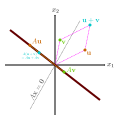
\includegraphics[width = 0.6\textwidth]{linear_mapping_range}
}
\end{tabular}

\textbf{Examples:}
\begin{itemize}
%%%%%%%%%%%%%%%%%%%%%%%%%%%%%%%
%%%%%%%% Example 1 
\item[1)] Let \[A = \begin{bmatrix}
  1 & 3 &  -1 &  -1 \\
  2 & 4 &   0 &   2 \\
-1 &  2 & -1 &   3 
\end{bmatrix}\]
It was previously determined that the row reduced form of \(A\) is:
\[A' = \begin{bmatrix}
1 & 0 & 0 & -3 \\
0 & 1 & 0 &  2 \\
0 & 0 & 1 &  4 
\end{bmatrix}\]
From the number of pivots, it can be seen that the number of linearly independent vectors that form the basis set of the range of \(A\) is \(3\). This means that \(\text{rank}(A) = 3\). It can also been seen from the number of free variable columns (the number of columns without pivots), that the dimension of the null space is \(\text{nullity}(A) = 1\). It can be observed that since the total number of columns is \(n = 4\), that:
\[4 = n = \text{rank}(A) + \text{nullity}(A) = 3 + 1\] 
%%%%%%%%%%%%%%%%%%%%%%%%%%%%%%%
%%%%%%%% Example 2 
\item[2)] Let \[A = \begin{bmatrix}
 1 &   1 &  2  &  -3 \\
-1 &   0 &  3 & -10 \\
 2 &   1 & -3 &  13 \\
-4 & -1 & 11 & -39
\end{bmatrix}\]
It was previously determined that the row reduced form of \(A\) is:
\[A' = \begin{bmatrix}
1 & 0 & 0 &  1 \\
0 & 1 & 0 &  2 \\
0 & 0 & 1 & -3 \\
0 & 0 & 0 &  0
\end{bmatrix}\]
From the number of pivots, it can be seen that the number of linearly independent vectors that form the basis set of the range of \(A\) is \(3\). This means that \(\text{rank}(A) = 3\). It can also been seen from the number of free variable columns (the number of columns without pivots), that the dimension of the null space is \(\text{nullity}(A) = 1\). It can be observed that since the total number of columns is \(n = 4\), that:
\[4 = n = \text{rank}(A) + \text{nullity}(A) = 3 + 1\] 
%%%%%%%%%%%%%%%%%%%%%%%%%%%%%%%
%%%%%%%% Example 3 
\item[3)] Let \[A = \begin{bmatrix}
 1 &  3 &  4 & -11 \\
-1 & -1 & 0 &    1 \\
 2 &  4 & 4 & -12 
\end{bmatrix}\]
It was previously determined that the row reduced form of \(A\) is: 
\[A' = \begin{bmatrix}
1 & 0 & -2 &  4 \\
0 & 1 &  2 & -5 \\
0 & 0 &  0 &  0 
\end{bmatrix}\]
From the number of pivots, it can be seen that the number of linearly independent vectors that form the basis set of the range of \(A\) is \(2\). This means that \(\text{rank}(A) = 2\). It can also been seen from the number of free variable columns (the number of columns without pivots), that the dimension of the null space is \(\text{nullity}(A) = 2\). It can be observed that since the total number of columns is \(n = 4\), that:
\[4 = n = \text{rank}(A) + \text{nullity}(A) = 2 + 2\] 
%%%%%%%%%%%%%%%%%%%%%%%%%%%%%%%
%%%%%%%% Example 4 
\item[4)] Let \[A = \begin{bmatrix}
-3 &   9 & -6 & -9 \\
-4 & 12 & -3 & -7 \\
 2 &  -6 &  0 &  2 \\ 
-1 &   3 &  1 &  0 \\
\end{bmatrix}\]
It was previously determined that the row reduced form of \(A\) is: 
\[A' = \begin{bmatrix}
1 & -3 & 0 & 1 \\
0 &  0 & 1 & 1 \\
0 &  0 & 0 & 0 \\ 
0 &  0 & 0 & 0
\end{bmatrix}\]
From the number of pivots, it can be seen that the number of linearly independent vectors that form the basis set of the range of \(A\) is \(2\). This means that \(\text{rank}(A) = 2\). It can also been seen from the number of free variable columns (the number of columns without pivots), that the dimension of the null space is \(\text{nullity}(A) = 2\). It can be observed that since the total number of columns is \(n = 4\), that:
\[4 = n = \text{rank}(A) + \text{nullity}(A) = 2 + 2\] 
%%%%%%%%%%%%%%%%%%%%%%%%%%%%%%%
%%%%%%%% Example 5 
\item[5)] Let \[A = \begin{bmatrix}
1 &  2 & -3 & -1 & -5 &  13 & 4 & -17 \\
1 &  1 & -1 &  0 &  1 &    9 &  2 &   -8 \\
0 &  1 & -2 &  1 &  4 &  10 &  0 &    3 \\
1 &  1 & -1 &  1 &  6 &  12 &  2 &   -8 \\ 
2 & -1 &  4 &  0 &  5 &  -3 &  1 &   -7 \\ 
\end{bmatrix}\]
It was previously determined that the row reduced form of \(A\) is: 
\[A' = \begin{bmatrix}
1 & 0 &  1 & 0 &  2 &  2 & 0 &  1 \\
0 & 1 & -2 & 0 & -1 & 7 & 0 &  3 \\
0 & 0 &  0 & 1 &  5 &  3 & 0 &  0 \\
0 & 0 &  0 & 0 &  0 &  0 & 1 & -6 \\ 
0 & 0 &  0 & 0 &  0 &  0 & 0 &  0 \\
\end{bmatrix}\]
From the number of pivots, it can be seen that the number of linearly independent vectors that form the basis set of the range of \(A\) is \(4\). This means that \(\text{rank}(A) = 4\). It can also been seen from the number of free variable columns (the number of columns without pivots), that the dimension of the null space is \(\text{nullity}(A) = 4\). It can be observed that since the total number of columns is \(n = 8\), that:
\[8 = n = \text{rank}(A) + \text{nullity}(A) = 4 + 4\] 
%%%%%%%%%%%%%%%%%%%%%%%%%%%%%%%
%%%%%%%% Example 6 
\item[6)] Let \[A = \begin{bmatrix}
-1 & -2 &  1 \\
 3 &  6 &  1 \\
 4 &  9 & -6 \\
-1 &  0 &  2 \\ 
\end{bmatrix}\]
It was previously determined that the row reduced form of \(A\) is: 
\[A' = \begin{bmatrix}
1 & 0 & 0 \\
0 & 1 & 0 \\
0 & 0 & 1 \\
0 & 0 & 0 \\ 
\end{bmatrix}\]
From the number of pivots, it can be seen that the number of linearly independent vectors that form the basis set of the range of \(A\) is \(3\). This means that \(\text{rank}(A) = 3\). It can also been seen from the number of free variable columns (the number of columns without pivots), that the dimension of the null space is \(\text{nullity}(A) = 0\). It can be observed that since the total number of columns is \(n = 3\), that:
\[3 = n = \text{rank}(A) + \text{nullity}(A) = 3 + 0\] 
%%%%%%%%%%%%%%%%%%%%%
%%%%%%%% Example 7 
\item[7)] Let \[A = \begin{bmatrix}
0 &  0 \\
0 &  1 \\
0 & -3 \\ 
0 &  2
\end{bmatrix}\]
It was previously determined that the row reduced form of \(A\) is: 
\[A' = \begin{bmatrix}
0 & 1 \\
0 & 0 \\
0 & 0 \\ 
0 & 0
\end{bmatrix}\] 
From the number of pivots, it can be seen that the number of linearly independent vectors that form the basis set of the range of \(A\) is \(1\). This means that \(\text{rank}(A) = 1\). It can also been seen from the number of free variable columns (the number of columns without pivots), that the dimension of the null space is \(\text{nullity}(A) = 1\). It can be observed that since the total number of columns is \(n = 2\), that:
\[2 = n = \text{rank}(A) + \text{nullity}(A) = 1 + 1\] 
%%%%%%%%%%%%%%%%%%%%%
%%%%%%%% Example 8 
\item[8)] Let \[A = \begin{bmatrix}
0 & 0 & 0 \\ 
0 & 0 & 0 \\ 
0 & 0 & 0 \\ 
0 & 0 & 0 \\ 
0 & 0 & 0 
\end{bmatrix}\]
The row reduced from of \(A\) is: 
\[A' = \begin{bmatrix}
0 & 0 & 0 \\ 
0 & 0 & 0 \\ 
0 & 0 & 0 \\ 
0 & 0 & 0 \\ 
0 & 0 & 0 
\end{bmatrix}\]
From the number of pivots, it can be seen that the number of linearly independent vectors that form the basis set of the range of \(A\) is \(0\). This means that \(\text{rank}(A) = 0\). It can also been seen from the number of free variable columns (the number of columns without pivots), that the dimension of the null space is \(\text{nullity}(A) = 3\). It can be observed that since the total number of columns is \(n = 3\), that:
\[3 = n = \text{rank}(A) + \text{nullity}(A) = 0 + 3\] 
\end{itemize}

%\section*{Functions revisited}
%
%Consider a function \(f\) with a domain of \(A\) and a co-domain of \(B\):
%
%\[f : A \rightarrow B\] 
%
%Given an arbitrary value of \(x\) from \(A\), \(f(x)\) is referred to as the ``image" of \(x\) under \(f\), or the ``output" of \(f\) given \(x\).
%
%The inverse \(f^{-1}\), if it exists, has a domain of \(B\) and a co-domain of \(A\):
%
%\[f^{-1} : B \rightarrow A\]
%
%For there to exist an inverse, one prerequisite is that the domain and co-domain have the same size:
%\[|A| = |B|\]
%
%If set \(A\) is larger than set \(B\), then there are guaranteed to exist two different values \(x_1\), \(x_2\) from \(A\) that yield the same output value \(f(x_1) = f(x_2)\).    



\end{document}










